\documentclass[a4paper,showframe,11pt]{report}
\usepackage{standalone}
\standalonetrue
\ifstandalone
  \usepackage{../../haziq_thesis}
  \usepackage{../../haziq_maths}
  \usepackage{../../haziq_glossary}
  \addbibresource{../../bib/haziq.bib}
  \externaldocument{../01/.texpadtmp/chapter1}
%  \externaldocument{../02/.texpadtmp/chapter2}  
  \externaldocument{../03/.texpadtmp/chapter3}
  \externaldocument{../04/.texpadtmp/chapter4}
  \externaldocument{../05/.texpadtmp/chapter5}
  \externaldocument{../06/.texpadtmp/chapter6}
  \externaldocument{../07/.texpadtmp/chapter7}
\fi

\begin{document}
\hChapterStandalone[2]{Vector space of functions}
\label{chapter2}

For regression modelling with I-priors, it is assumed that the regression functions lie in some vector space of functions.
The purpose of this chapter is to provide a concise review of functional analysis leading up to the theory of reproducing kernel Hilbert and Kreĭn spaces (RKHS/RKKS).
The interest with these RKHSs and RKKSs is that these spaces have well established mathematical structure and offer desirable topologies.
In particular, it allows the possibility of deriving the Fisher information for regression functions---this will be covered in \cref{chapter3}.
As we shall see, RKHSs are also extremely convenient in that they may be specified completely via their reproducing kernels.
Several of these function spaces are of interest to us, for example, spaces of linear functions, smoothing functions, and functions whose inputs are nominal values and even functions themselves.
RKHSs are widely studied in the applied statistical and machine learning literature, but perhaps RKKSs are less so.
To provide an early insight, RKKSs are simply a generalisation of RKHSs, and are defined as the difference between two RKHSs.
The flexibility provided by RKKSs will prove both useful and necessary, especially when considering sums and products of scaled function spaces, as is done in I-prior modelling.

It is emphasised that a deep knowledge of functional analysis, including RKHS and RKKS theory, is not at all necessary for I-prior modelling, so perhaps the advanced reader may wish to skip \cref{sec:funcanalysis,sec:rkhstheory,sec:rkkstheory}. 
\cref{sec:rkhsbuild} describes the fundamental RKHS of interest for I-prior regression, which we refer to as the ``building block'' RKHSs.
The reason for this is that it is possible to construct new function spaces from existing ones, and this is described in \cref{sec:constructrkks}.

Two remarks before starting.
Firstly, on notation: sets and vector spaces are denoted by calligraphic letters, and as much as possible, we shall stick to the convention that $\cF$ denotes a function space, and $\cX$ denotes the set of covariates or function inputs. 
Occasionally, we will describe a generic Hilbert space denoted by $\cH$.
Elements of the vector space of real functions over a set $\cX$ are denoted $f(\cdot)$, but more commonly and simply $f$.
This distinguishes them from the actual evaluation of the function at an input point $x \in \cX$, denoted $f(x) \in \bbR$.
For a much cleaner read, we dispense with boldface notation for vectors and matrices when talking about them, without ambiguity, in the abstract sense.
Secondly, on bibliography: references will be minimised throughout the presentation of this chapter, but a complete annotated bibliography at the end in \cref{sec:summarychapter2}.
 
%A vector space... of `functions'?
%
%At first glance, this may seem strange, that the notion of functions (as mappings from input to output space) and vector spaces are somehow equatable.
%Upon further thought, one realises that firstly, two functions of a similar, particular form may be added together (in some meaningful way) resulting in a function in that same form. 
%Secondly, multiplication of a function by a scalar $c$ can be thought of as $c$ times the output of that function.
%Indeed, running through the checklist of what constitutes a vector space, we find that a ``space of functions'' satisfies them all.
%In modern linear algebra texts, this checklist is the eight axioms of vector spaces over a field $\bbF$: The vectors forms an abelian group under addition, and this group has an $\bbF$-module structure.

\section{Some functional analysis}\label{sec:funcanalysis}
\index{vector space}
\index{linear space|see {vector space}}
\index{inner product}
The core study of functional analysis revolves around the treatment of functions as objects in vector spaces over a field\footnote{In this thesis, this will be $\bbR$ exclusively.}.
Vector spaces, or linear spaces as they are sometimes known, may be endowed with some kind of structure so as to allow ideas such as closeness and limits to be conceived.
Of particular interest to us is the structure brought about by \emph{inner products}\index{inner product}, which allow the rigorous mathematical study of various geometrical concepts such as lengths, directions, and orthogonality, among other things.
We begin with the definition of an inner product. 

\begin{definition}[Inner products]\label{def:innerprod}
	Let $\mathcal F$ be a vector space over $\mathbb R$. A function $\langle\cdot,\cdot\rangle_{\mathcal F}:\mathcal F \times \mathcal F \rightarrow \mathbb R$ is said to be an inner product on $\mathcal F$ if all of the following are satisfied:
	\begin{itemize}
	\item \textbf{Symmetry}. $\langle f, g\rangle_{\mathcal F} = \langle g, f \rangle_{\mathcal F}$, $\forall f,g \in \mathcal F$.
	\item \textbf{Linearity}. $\langle \lambda_1 f_1 + \lambda_2 f_2, g\rangle_{\mathcal F} = \lambda_1\langle f_1,g \rangle_{\mathcal F} + \lambda_2\langle f_2,g \rangle_{\mathcal F}$, $\forall f_1, f_2, g \in \mathcal F$, $\forall \lambda_1,\lambda_2 \in \mathbb R$.
	\item \textbf{Non-degeneracy}. $\langle f, f\rangle_{\mathcal F} = 0 \Leftrightarrow f=0$.
	\end{itemize}
\end{definition}

\index{inner product!positive-definite}
Additionally, an inner product is said to be \emph{positive definite} if $\langle f, f\rangle_{\mathcal F} \geq 0$, $\forall f \in \mathcal F$.
Inner products need not necessarily be positive definite, and we shall revisit this fact later when we cover Kreĭn spaces.
For the purposes of the forthcoming discussion, the inner products that are referenced are the positive-definite kind, unless otherwise stated.

\index{norm}
We can always define a \emph{norm} on $\cF$ using the inner product as 
\begin{equation}\label{eq:normip}
  \norm{f}_\cF = \sqrt{\ip{f,f}_\cF}.
\end{equation}
Norms are another form of structure that specifically captures the notion of length. 
This is defined below.

\begin{definition}[Norms]
	Let $\mathcal F$ be a vector space over $\mathbb R$. A non-negative function $||\cdot||_{\mathcal F}:\mathcal F \times \mathcal F \rightarrow \mathbb [0,\infty)$ is said to be a norm  on $\mathcal F$ if all of the following are satisfied:
	\begin{itemize}
	\item \textbf{Absolute homogeneity}. $||\lambda f||_{\mathcal F} = |\lambda| \, ||f||_{\mathcal F}$, $\forall \lambda \in \mathbb R$, $\forall f \in \mathcal F$
	\item \textbf{Subadditivity}. $||f+g||_{\mathcal F} \leq ||f||_{\mathcal F} + ||g||_{\mathcal F}$, $\forall f,g \in \mathcal F$
	\item \textbf{Point separating}. $||f||_{\mathcal F} = 0 \Leftrightarrow f=0$
	\end{itemize}
	Note that since $\norm{-f}_\cF = \abs{-1} \, \norm{f}_\cF = \norm{f}_\cF$, and by the subadditivity and point separating property, we have that $\norm{f}_\cF = \half\norm{f}_\cF + \half\norm{-f}_\cF \geq \half\norm{f - f}_\cF = 0$, thus implying non-negativity of norms.
\end{definition}


\index{triangle inequality}
\index{reverse triangle inequality}
\index{Cauchy-Schwarz inequality}
\index{parallelogram law}
\index{polarisation identity}
The subadditivity property is also known as the \emph{triangle inequality}.
Following this, there is also the \emph{reverse triangle inequality}, which states $\norm{f-g}_\cF \geq \big\vert \norm{f}_\cF - \norm{g}_\cF \big\vert$.
In fact, the general forms of these triangle inequalities \citep[Lemma 10]{bergsma2017} also hold for $0\leq a\leq 1$ and any $f,g,h\in\cF$:
\newcommand{\normF}[1]{\norm{#1}_\cF}
\begingroup
\setlength{\abovedisplayskip}{9pt}
\setlength{\belowdisplayskip}{7pt}
\begin{align}
  \normF{f-g}^a &\leq \normF{f-h}^a + \normF{g-h}^a \label{eq:trieq1} \\ 
  \normF{f-g}^a &\geq \big\vert \normF{f}^a - \normF{g}^a \big\vert. \label{eq:trieq2}
\end{align}
\endgroup
Several other important relationships involving norms and inner products hold in linear spaces, namely, the \emph{Cauchy-Schwarz inequality}
\begingroup
\setlength{\abovedisplayskip}{9pt}
\setlength{\belowdisplayskip}{7pt}
\[
  |\ip{f,g}_\cF| \leq \norm{f}_\cF \, \norm{g}_\cF;
\]
\endgroup
the \emph{parallelogram law}
\begingroup
\setlength{\abovedisplayskip}{7pt}
\setlength{\belowdisplayskip}{7pt}
\[
  \norm{f+g}_\cF^2 + \norm{f-g}_\cF^2 = 2\norm{f}_\cF^2 + 2\norm{g}_\cF^2;
\]
\endgroup
and the \emph{polarisation identity} (in various forms)
\begingroup
\setlength{\abovedisplayskip}{9pt}
\setlength{\belowdisplayskip}{7pt}
\begin{align*}
  \norm{f+g}_\cF^2 - \norm{f-g}_\cF^2 &= 4\ip{f,g}_\cF,  \\
  \norm{f+g}_\cF^2 - \norm{f}_\cF^2 - \norm{g}_\cF^2 &= 2\ip{f,g}_\cF, \\
  - \norm{f-g}_\cF^2 + \norm{f}_\cF^2 + \norm{g}_\cF^2  &= 2\ip{f,g}_\cF,
\end{align*}
\endgroup
for any $f,g\in\cF$.

A vector space endowed with an inner product (c.f. norm) is called an inner product space (c.f. normed vector space).
As a remark, inner product spaces can always be equipped with a norm using \cref{eq:normip}, but not always the other way around.
A norm needs to satisfy the parallelogram law for an inner product to be properly defined.

\index{metric}
\index{convergence}
\index{Cauchy sequence}
The norm $||\cdot||_{\mathcal F}$, in turn, induces a metric (a notion of distance) on $\mathcal F$, i.e. $D(f,g) = ||f-g||_{\mathcal F}$, for $f,g\in\cF$.
With these notions of distances, one may talk about sequences of functions in $\cF$ which are \emph{convergent}, and sequences whose elements become arbitrarily close to one another as the sequence progresses (\emph{Cauchy}).

\begin{definition}[Convergent sequence]
	A sequence $\{f_n\}_{n=1}^\infty$ of elements of a normed vector space $(\mathcal F, ||\cdot ||_{\mathcal F})$ is said to \emph{converge} to some $f\in\cF$, if for every $\epsilon > 0$, $\exists N=N(\epsilon) \in \mathbb N$, such that $\forall n > N$, $||f_n - f||_{\mathcal F} < \epsilon$.
\end{definition}

\begin{definition}[Cauchy sequence]
	A sequence $\{f_n\}_{n=1}^\infty$ of elements of a normed vector space $(\mathcal F, ||\cdot ||_{\mathcal F})$ is said to be a Cauchy sequence if for every $\epsilon > 0$, $\exists N=N(\epsilon) \in \mathbb N$, such that $\forall n,m > N$, $||f_n - f_m||_{\mathcal F} < \epsilon$.
\end{definition}

\index{vector space!complete}
\index{Hilbert space}
\index{Banach space}
\index{Hilbert space!pre-Hilbert space}
Every convergent sequence is Cauchy (from the triangle inequality), but the converse is not true.
If the limit of the Cauchy sequence exists within the vector space, then the sequence converges to it.
A vector space is said to be \emph{complete} if it contains the limits of all Cauchy sequences, or in other words, if every Cauchy sequence converges.
There are special names given to complete vector spaces.
A complete inner product space is known as a \emph{Hilbert space}, while a complete normed space is called a \emph{Banach space}.
Out of interest, an inner product space that is not complete is sometimes known as a \emph{pre-Hilbert space}, since its completion with respect to the norm induced by the inner product is a Hilbert space.

\index{closed subspace}
A subset $\cG\subseteq\cF$ is a \emph{closed subspace} of $\cF$ if it is closed under addition and multiplication by a scalar.
That is, for any $g,g'\in\cG$, $\lambda_1 g + \lambda_2 g'$ is also in $\cG$, for $\lambda_1,\lambda_2\in\bbR$.
For Hilbert spaces, each closed subspace is also complete, and thus a Hilbert space in its own right.
Although, as a remark, not every Hilbert subspace need be closed, and therefore complete. 

\index{operator!linear|see{linear map}}
\index{operator!bilinear|see{bilinear map}}
\index{linear!map}
\index{linear!functional}
\index{bilinear!map}
\index{bilinear!form}
Being vectors in a vector space, we can discuss mapping of vectors onto a another space, or in essence, having a function acted upon them.
To establish terminology, we define linear and bilinear maps (operators).

\begin{definition}[Linear map/operator]
  Let $\cF$ and $\cG$ be two Hilbert spaces over $\bbR$.
  An operator $A$ is a map from $\cF$ to $\cG$, and we denote its action on a function $f \in\cF$ as $A(f) \in \cG$, or simply $Af \in \cG$.
  A \emph{linear operator} satisfies $A(f+f') = A(f) + A(f')$ and $A(\lambda f) = \lambda A(f)$, for all $f,f' \in\cF$ and $\lambda\in\bbR$.
  If $\cG$ is the base field ($\bbR$ in our case), then the linear operator $A$ is called a \emph{linear functional}.
\end{definition}

\begin{definition}[Bilinear map/operator]
  Let $\cF$, $\cG$ and $\cH$ be Hilbert spaces over $\bbR$.
  A \emph{bilinear operator} $B:\cF\times\cG\to\cH$ is linear in each argument separately, i.e.
  \begin{itemize}
    \item $B(\lambda_1 f +\lambda_2 f', h) = \lambda_1 B(f,h) + \lambda_2 B(f',h)$; and
    \item $B(f, \lambda_1 g +\lambda_2 g') = \lambda_1 B(f,g) + \lambda_2 B(f,g')$,
  \end{itemize} 
  for all $f,f' \in \cF$, $g,g' \in \cG$ and $\lambda_1,\lambda_2\in\bbR$.
  In other words, the mappings $B_g: f \mapsto B(f,g)$ for any $g\in\cG$, and $B_f: g \mapsto B(f,g)$ for any $f\in\cF$, are both linear maps.
  If $\cF\equiv\cG$, then the bilinear map is \emph{symmetric}.
  If $\cH$ is the base field ($\bbR$ in our case), then $B$ is called a \emph{bilinear form}.
\end{definition}

\vspace{-0.6em}
An interesting property of these operators to look at, besides linearity, is whether or not they are \emph{continuous}.

\begin{definition}[Continuity]\label{def:continuity}
  \index{continuity}
  \index{continuity!uniform}
  \index{uniformly continuous}
  \index{uniformly continuous|seealso{continuity}}
  Let $\cF$ and $\cG$ be two Hilbert spaces.
  A function $A:\cF\to\cG$ is said to be \emph{continuous at $g\in\cF$}, if for every $\epsilon>0$, $\exists \delta=\delta(\epsilon,g)>0$ such that
  \[
    \norm{f-g}_\cF < \delta \ \ \Rightarrow \ \ \norm{Af - Ag}_\cG < \epsilon.
  \]
  A is \emph{continuous} on $\cF$, if it is continuous at every point $g \in\cF$.
  If, in addition, $\delta$ depends on $\epsilon$ only, $A$ is said to be \emph{uniformly continuous}.
\end{definition}

Continuity in the sense of linear operators here means that a convergent sequence in $\cF$ can be mapped to a convergent sequence in $\cG$.
For a particular linear operator, the evaluation functional, this means that closeness in norm implies pointwise closeness---this relates to RKHSs, which is discussed in \cref{sec:rkhstheory}.
There is an even stronger notion of continuity called  \emph{Lipschitz continuity}.

\index{Lipschitz continuous|seealso{continuity}}
\index{Lipschitz continuous}
\index{continuity!Lipschitz}
\begin{definition}[Lipschitz continuity]
  Let $\cF$ and $\cG$ be two Hilbert spaces.  
  A function $A:\cF\to\cG$ is \emph{Lipschitz continuous} if $\exists M >0$ such that $\forall f,f'\in\cF$,
  \[
    \norm{Af - Af'}_\cG \leq M \norm{f - f'}_\cF.
  \]
\end{definition}

\vspace{-0.75em}
Clearly, Lipschitz continuity implies uniform continuity: choose $\delta = \delta(\epsilon) := \epsilon/M$ and replace this in  \cref{def:continuity}.
A continuous, linear operator is also one that is bounded.

\index{operator!bounded}
\index{bounded}
\begin{definition}[Bounded operator]\label{def:boundedop}
  The linear operator $A:\mathcal F \rightarrow \mathcal G$ between two Hilbert spaces $\cF$ and $\cG$ is said to be \emph{bounded} if there exists some $M>0$ such that
  \[
    \norm{Af}_\cG \leq M \norm{f}_\cF.\vspace{-0.4em}
  \]
  The smallest such $M$ is defined to be the \emph{operator norm}, denoted $\norm{A} := \sup_{f\in\cF} \frac{\norm{Af}_\cG}{\norm{f}_\cF}$.
\end{definition}

\begin{lemma}[Equivalence of boundedness and continuity]\label{thm:boundcont}
  Let $\cF$ and $\cG$ be two Hilbert spaces, and $A:\cF\to\cG$ a linear operator.
  $A$ is bounded if and only if it is continuous.
\end{lemma}

\begin{proof}
  Suppose that $A$ is bounded.
  Then, $\forall f,f' \in \cF$, $\exists M>0$ such that $\norm{A(f-f')}_\cG \leq M \norm{f-f'}_\cG$, so $A$ is Lipschitz continuous.
  Conversely, let $A$ be a continuous linear operator, especially at the zero vector.
  In other words, $\exists \delta > 0$ such that $\norm{A(f)}_\cG = \norm{A(f+0-0)}_\cG = \norm{A(f) - A(0)} \leq 1$, $\forall f\in\cF$ whenever $\norm{f}_\cF \leq \delta$.
  Thus, for all non-zero $f \in\cF$,
  \begingroup
  \setlength{\abovedisplayskip}{7pt}
  \setlength{\belowdisplayskip}{7pt}
  \begin{align*}
    \norm{A(f)}_\cG &= \left\Vert \frac{\norm{f}_\cF}{\delta} A\left(\frac{\delta}{\norm{f}_\cF}f\right)\right\Vert_\cG \\
    &= \left\vert \frac{\norm{f}_\cF}{\delta}\right\vert \, \left\Vert A\left(\frac{\delta}{\norm{f}_\cF}f\right)\right\Vert_\cG \\    
    &\leq \frac{\norm{f}_\cF}{\delta} \cdot 1,
  \end{align*}
  \endgroup
  and therefore $A$ is bounded.
\end{proof}
\vspace{-0.5em}
So important is the concept of linearity and continuity, that there are specially named spaces which contain linear and continuous functionals.

\index{dual space!algebraic dual}
\index{dual space!continuous dual}
\begin{definition}[Dual spaces]
  Let $\cF$ be a Hilbert space. 
  The space $\cF^\vee$ of \emph{linear functionals} is called the \emph{algebraic dual space} of $\cF$.
  The space $\cF^*$ of \emph{continuous linear functionals} is called the \emph{continuous dual space} or alternatively, the \emph{topological dual space}, of $\cF$.   
\end{definition}

As it turns out, the algebraic dual space and continuous dual space coincide in finite-dimensional Hilbert spaces:
take any $A\in\cF^\vee$; since $A$ is finite-dimensional, it is bounded, and therefore continuous (see \cref{thm:boundcont}), so $A\in\cF^*$ and $\cF^\vee \subseteq \cF^*$; but $\cF^* \subseteq \cF^\vee$ trivially, so $\cF^\vee \equiv \cF^*$.
For infinite-dimensional Hilbert spaces, this is not so, but in any case, we will only be considering the continuous dual space in this thesis.
The following result is an important one, which states that continuous linear functionals of an inner product space are nothing more than inner products.

\index{Riesz-Fréchet theorem|see{Riesz representation theorem}}
\begin{theorem}[Riesz-Fréchet]
  \index{Riesz representation theorem}
  Let $\cF$ be a Hilbert space.
  Every element $A$ of the continuous dual space $\cF^*$, i.e. all continuous linear functionals $A:\cF\to\bbR$, can be uniquely written in the form $\ip{\cdot,g}_\cF =: A_g \in \cF^*$, for some $g\in\cF$. 
  Moreover, $\norm{g}_\cF = \norm{A_g}_{\cF^*}$.
\end{theorem}

\begin{proof}
  Omitted---see \citet[Theorem 4.2.1]{yamamoto2012vector} for a proof.
%  \citet[Theorem 4.12]{rudin1987real} 
\end{proof}

\begin{remark}
  The Riesz-Fréchet theorem is also commonly referred to as the \emph{Riesz representation theorem} for Hilbert spaces.
\end{remark}

\index{isometry}
\index{isomorphism}
The notion of isometry (transformation that preserves distance) is usually associated with metric spaces; two metric spaces being isometric means that they identical as far as their metric properties are concerned.
For Hilbert spaces (and more generally, for normed spaces), there is an analogous concept as well in \emph{isometric isomorphism} (a bijective isometry), such that two Hilbert spaces being isometrically isomorphic imply that they have exactly the same geometric structure, but may very well contain fundamentally different objects.

\begin{definition}[Isometric isomorphism]
  Two Hilbert spaces $\cF$ and $\cG$ are said to be \emph{isometrically isomorphic}, symbolised $\cF \cong \cG$, if there is a linear bijective map $U:\cF\to\cG$ which preserves the inner product, i.e. for any $f,f'\in\cF$, 
  \[
    \ip{f,f'}_\cF = \ip{Uf,Uf'}_\cG.
  \]
\end{definition}

A consequence of the Riesz-Fréchet theorem is that it gives us a canonical isometric isomorphism $U:g\mapsto \ip{\cdot,g}_\cF =: A_g$ between $\cF$ and its continuous dual $\cF^*$:
the map $A_g$ is obviously linear (by the bilinear property of inner products), and using the polarisation identity, we have that
\begin{align*}
  2\ip{Ug,Ug'}_{\cF^*} 
  &= \norm{U(g)}_{\cF^*}^2 + \norm{U(g')}_{\cF^*}^2 - \norm{U(g - g')}_{\cF^*}^2 \\
  &= \norm{g}_{\cF}^2 + \norm{g'}_{\cF}^2 - \norm{g-g'}_{\cF}^2 \\
  &= 2\ip{g,g'}_{\cF}.
\end{align*}
%An isometry that preserves the norm is known as \emph{linear isometry}.
Implicitly, this means that $\cF^*$ is a Hilbert space as well.

\index{orthogonal!projection}
\index{orthogonal!complement}
\index{orthogonal!decomposition}
\index{polarisation identity}
Another important type of mapping is the mapping $P$ of an element in $\cF$ onto a closed subspace $\cG\subset\cF$, such that $Pf \in \cG$ is closest to $f$.
This mapping is called the \emph{orthogonal projection}, due to the fact that such projections yield perpendicularity in the sense that $\ip{f-Pf,g}_\cF = 0$ for any $g\in\cG$.
Consequently, we see that $\norm{f}_\cF^2 = \norm{Pf}_\cF^2 + \norm{f-Pf}_\cF^2$ from the polarisation identity.
The remainder $f - Pf$ belongs to the \emph{orthogonal complement} of $\cG$.
%The remainder $f - Pf = (I-P)f = Qf$, where $I$ is the identity map, belongs to the \emph{orthogonal complement} of $\cG$.
%As a consequence, $\norm{f}_\cF^2 = \norm{Pf}_\cF^2 + \norm{Qf}_\cF^2$.

\begin{definition}[Orthogonal complement]
  Let $\cF$ be a Hilbert space and $\cG \subset \cF$ be a closed subspace.
  The linear subspace $\cG^\bot = \{ f \,|\, \ip{f,g}_\cF = 0, \forall g \in \cG \}$ is called the orthogonal complement of $\cG$ in $\cF$.
\end{definition}

\begin{theorem}[Orthogonal decomposition]\label{thm:orthdecomp}
  Let $\cF$ be a Hilbert space and $\cG \subset \cF$ be a closed subspace.
  For every $f \in \cF$, we can write $f = g + g^c$, where $g \in \cG$ and $g^c \in \cG^\bot$, and this decomposition is unique.
\end{theorem}

\begin{proof}
  Omitted---see \citet[Theorem 4.11]{rudin1987real} for a proof.
\end{proof}

\index{tensor!sum}
We can write $\cF = \cG \oplus \cG^\bot$, where the $\oplus$ symbol denotes the \emph{direct sum}, and such a decomposition is called a \emph{tensor sum decomposition}.
In infinite-dimensional Hilbert spaces, some subspaces are not closed, but all orthogonal complements are closed. 
In such spaces, the orthogonal complement of the orthogonal complement of $\cG$ is the closure of $\cG$, i.e. $(\cG^\bot)^\bot =: \overline \cG$, and we say that $\cG$ is \emph{dense} in $\overline \cG$.
Another interesting fact regarding the orthogonal complement is that $\cG \cap \cG^\bot = \{ 0 \}$, since any $g\in \cG \cap \cG^\bot$ must be orthogonal to itself, i.e. $\ip{g,g}_\cG = 0$ implying that $g=0$.

The following theorem states that orthogonal decompositions are unique.

\begin{corollary}\label{thm:orthdecomp2}
  Let $\cG$ be a subspace of a Hilbert space $\cF$. 
  Then, $\cG^\bot = \{0\}$ if and only if $\cG$ is dense in $\cF$.
\end{corollary}

\begin{proof}
  If $\cG^\bot=\{0\}$ then $(\cG^\bot)^\bot = \overline \cG = \cF$.
  Conversely, since $\cG$ is dense in $\cF$, we have $\cG^\bot = \overline\cG^\bot = \cF^\bot = \{0\}$.
%  Conversely, suppose that there exists a non-zero element $h \in \cG^\bot$.
%  Because $\cG$ is dense, we can construct a sequence $\{h_n\}_{n=1}^\infty\in\cG$ converging to $h$.
%  We have
%  \begin{align*}
%    \norm{h}_\cG^2 
%    &= \ip{h,h}_\cG \\
%    &= \ip{h,h}_\cG - \ip{h_n,h}_\cG \hspace{1em} \rlap{\color{grymath} since $h$ is in $\cG^\bot$} \\
%    &= \ip{h-h_n,h}_\cG \\
%    &\leq \norm{h-h_n}_\cG \cdot \norm{h}_\cG,
%  \end{align*}
%  but the final term tends to zero since $h_n$ converges to $h$.
%  So $h=0$, a contradiction.
\end{proof}

%https://en.wikibooks.org/wiki/Functional_Analysis/Hilbert_spaces

Besides tensor sums, of importance is the concept of \emph{tensor products}, which can be thought of as a generalisation of the outer product in Euclidean space.

\index{tensor!product}
\begin{definition}[Tensor products]\label{def:tensorprod}
  Let $x_1\in\cH_1$ and $x_2\in\cH_2$ be two elements of two real Hilbert spaces.
  Then, the tensor product $x_1 \otimes x_2:\cH_1\times\cH_2\to\bbR$, is a bilinear form defined as
  \begingroup
  \setlength{\abovedisplayskip}{3pt}
  \setlength{\belowdisplayskip}{5pt}
  \[
    (x_1\otimes x_2)(y_1,y_2) = \ip{x_1,y_1}_{\cH_1}\ip{x_2,y_2}_{\cH_2}
  \]
  \endgroup
  for any $(y_1,y_2)\in\cH_1\times\cH_2$.
\end{definition}

Correspondingly, we may also define the \emph{tensor product space}.

\index{tensor!product space}
\begin{definition}[Tensor product space]\label{def:tensprodspace}
  The tensor product space $\cH_1\otimes\cH_2$ is the completion of the space
  \begingroup
  \setlength{\abovedisplayskip}{8pt}
  \setlength{\belowdisplayskip}{8pt}
  \[
    \cA = \left\{ \sum_{j=1}^J x_{1j} \otimes x_{2j} \,\Bigg\vert\, x_{1j}\in\cH_1, x_{2j}\in\cH_2, J \in \bbN \right\}.
  \]
  \endgroup
  with respect to the norm induced by the inner product
  \[
    \left\langle  \sum_{j=1}^J x_{1j} \otimes x_{2j},  \sum_{k=1}^K y_{1k} \otimes y_{2k} \right\rangle_\cA = \sum_{j=1}^J\sum_{k=1}^K \ip{x_{1j},y_{1k}}_{\cH_1} \ip{x_{2j},y_{2k}}_{\cH_2}.
  \]
\end{definition}

\index{operator!rank one}
\index{operator!tensor product}
\index{bilinear!form}
Interestingly, the tensor product can be viewed as an operator between two Hilbert spaces.
That is, for each pair of elements $(x_1,x_2) \in \cH_1\times\cH_2$, we define the operator $A_{x_1,x_2}:\cH_1\to\cH_2$ in the following way:
\begingroup
\setlength{\abovedisplayskip}{7pt}
\setlength{\belowdisplayskip}{7pt}
\begin{align*}
  A_{x_1,x_2}:\cH_1&\to\cH_2 \\
  y_1&\mapsto \ip{x_1,y_1}_{\cH_1}x_2.
\end{align*}
\endgroup
Incidentally, an operator defined in such a way is called a \emph{rank one} operator.
Indeed, for some $y_1\in\cH_1$ and $y_2\in\cH_2$, we have that
\begingroup
\setlength{\abovedisplayskip}{7pt}
\setlength{\belowdisplayskip}{6pt}
\begin{align*}
  \ip{A_{x_1,x_2}(y_1),y_2}_{\cH_2} 
  &= \big\langle \ip{x_1,y_1}_{\cH_1}x_2 , y_2 \big\rangle_{\cH_2} \\
  &= \ip{x_1,y_1}_{\cH_1}\ip{x_2,y_2}_{\cH_2} \\
  &= (x_1\otimes x_2)(y_1,y_2). 
\end{align*}
\endgroup
We now have three distinct interpretations of the tensor product.
For $x_1,y_1\in\cH_1$ and $x_2,y_2\in\cH_2$, these are:
\begingroup
\setlength{\abovedisplayskip}{5pt}
\setlength{\belowdisplayskip}{5pt}
\begin{itemize}
  \item \textbf{General form}. An element in the tensor product space
  \[
    x_1 \otimes x_2 \in \cH_1 \otimes \cH_2 
  \]
  \item \textbf{Operator form}. An operator between two Hilbert spaces
  \begin{align*}
    x_1 \otimes x_2:\cH_1 &\to \cH_2 \\
    y_1 &\mapsto \ip{x_1,y_1}_{\cH_1}x_2 
  \end{align*}  
  \item \textbf{Bilinear form}. As per \cref{def:tensorprod}
  \begin{align*}
    x_1 \otimes x_2:\cH_1 \times \cH_2 &\to \bbR \\
    (y_1,y_2) &\mapsto \ip{x_1,y_1}_{\cH_1}\ip{x_2,y_2}_{\cH_2}
  \end{align*}
\end{itemize}
\endgroup

\begin{remark}
  As explained by \citet[sec. 10.5, p. 227]{kokoszka2017introduction}, tensors are often thought of as generalisations of matrices.
  For example, in Euclidean space, a matrix $\bA \in \bbR^{n\times m}$, formed by two vectors $x_1\in\bbR^n$ and $x_2\in\bbR^m$ via $\bA = x_1x_2^\top =: x_1 \otimes x_2$, can be viewed in at least three ways: 
  1) as a traditional matrix in the space $\bbR^n \otimes \bbR^m = \bbR^{n\times m}$; 
  2) as a linear operator in Euclidean space $\bA:\bbR^n\to\bbR^m$ (or the reverse) by multiplying $\bA$ from the left or right by a vector; or
  3) as a bilinear mapping $\bA:\bbR^n \times \bbR^m \to \bbR$ in the form of $\bA(y_1,y_2) = y_1^\top\bA y_2 = y_1^\top x_1 x_2^\top y_2 = (y_1^\top x_1)(y_2^\top x_2)$, for some $y_1\in\bbR^n$ and $y_2\in\bbR^m$, arising often in the study of quadratic forms.
\end{remark}

\index{sigma algebra|seealso{Borel space}}
\index{sigma algebra}
\index{Borel space}
For the last part of this introductory section on functional analysis, we discuss measures on Hilbert spaces, and in particular, a probability measure.
Let $\cH$ be a real Hilbert space. 
As discussed earlier, we can define a metric on $\cH$ using $D(x,x') = \norm{x-x'}_\cH$, where the norm on $\cH$ is the norm induced by the inner product.
A collection $\Sigma$ of subsets of $\cH$ is called a \emph{$\sigma$-algebra} if $\emptyset \in \Sigma$, $S \in \Sigma$ implies its complement $S^c \in \Sigma$, and $S_j\in\Sigma$, $j\geq 1$ implies $\bigcup_{j=1}^\infty S_j \in \Sigma$.
The smallest $\sigma$-algebra containing all open subsets of $\cH$ is called the \emph{Borel $\sigma$-algebra}, and its members the Borel sets.
Denote by $\cB(\cH)$ the Borel $\sigma$-algebra of $\cH$.
%The metric space $(\cH,D)$ is called \emph{separable} if it has a countable dense subset, i.e., there are $x_1,x_2,\cdots$ in $\cH$ such that the closure $\overline{\{x,_1,x_2,\cdots\}} = \cH$.

Recall that a function $\nu:\Sigma\to[0,\infty]$ is called a \emph{measure} if it satisfies
\begin{itemize}
  \item \textbf{Non-negativity:} $\nu(S) \geq 0$ for all $S$ in $\Sigma$;
  \item \textbf{Null empty set:} $\nu(\emptyset) = 0$; and
  \item \textbf{$\sigma$-additivity:} for all countable, mutually disjoint sets $\{S_i\}_{i=1}^\infty$,
  \[
    \nu\left(\bigcup_{i=1}^\infty S_i \right) = \sum_{i=1}^\infty \nu(S_i).
  \] 
\end{itemize}
A measure $\nu$ on $\big(\cH,\cB(\cH)\big)$ is called a \emph{Borel measure} on $\cH$.
We shall only concern ourselves with finite Borel measures. 
In addition, if $\nu(\cH) = 1$ then $\nu$ is a \emph{(Borel) probability measure} and the measure space $\big(\cH,\cB(\cH),\nu\big)$ is a \emph{(Borel) probability space}.

\index{random element}
\index{distribution}
\index{density}
Let $(\Omega,\cE,\Prob)$ be a probability space.
We say that a mapping $X:\Omega\to\cH$ is a \emph{random element} in $\cH$ if $X^{-1}(B)\in\cE$ for every Borel set, i.e., $X$ is a function such that for every $B\in\cB(\cH)$, its preimage $X^{-1}(B) = \{\omega \in \Omega \,|\, X(\omega) \in B \}$ lies in $\cE$.
This is simply a generalisation of the definition of random variables in regular Euclidean space.
From this definition, we can also properly define random functions $f$ in a Hilbert space of functions $\cF$.
In any case, every random element $X$ induces a probability measure on $\cH$ defined by
\[
  \nu(B) = \Prob\big(X^{-1}(B)\big) = \Prob\big( \omega \in \Omega | X(\omega) \in B  \big) = \Prob(X \in B).
\]
The measure $\nu$ is called the \emph{distribution} of $X$.
The \emph{density} $p$ of $X$ is a measurable function with the property that
\begingroup
\setlength{\abovedisplayskip}{7pt}
%\setlength{\belowdisplayskip}{5pt}
\[
  \Prob(X \in B) = \int_{X^{-1}(B)} \omega \dint\Prob(\omega) = \int_B p(x) \dint\nu(x).
\]
\endgroup

\begin{definition}[Mean vector]
  \index{mean vector}
  Let $\nu$ be a Borel probability measure on a real Hilbert space $\cH$.
  Supposing that a random element $X$ of $\cH$ is \emph{integrable}, that is to say
  \[
    \E \norm{X}_\cH = \int_\cH \norm{z}_\cH \dint\nu(z) < \infty,
  \]
  then the unique element $\mu\in\cH$ satisfying 
  \[
    \ip{\mu,x} = \int_\cX \ip{z,x}_\cX \dint\nu(z) = \E\ip{X,x}_\cH
  \]
  for all $x \in \cH$ is called the \emph{mean vector}. 
\end{definition}

\begin{definition}[Covariance operator]\label{def:covoper}
  \index{covariance operator}
  \index{operator!covariance|see{covariance operator}}
  Let $\nu$ be a Borel probability measure on a real Hilbert space $\cH$.
  Suppose that a random element $X$ of $\cH$ is \emph{square integrable}, i.e., $\E \norm{X}_\cH^2 < \infty$, and let $\mu$ be the mean vector of $X$.
  Then the \emph{covariance operator} $C$ is defined by the mapping
  \begingroup
  \setlength{\abovedisplayskip}{4pt}
  \setlength{\belowdisplayskip}{6pt}
  \begin{align*}
    C:\cH &\to \cH \\
    x &\mapsto \E\big[\ip{X - \mu, x}_{\cH}(X - \mu) \big].
  \end{align*}
  \endgroup
  The covariance operator $C$ is also an element of $\cH\otimes\cH$ that satisfies
  \begingroup
  \setlength{\abovedisplayskip}{13pt}
  \setlength{\belowdisplayskip}{4pt} 
  \begin{align*}
    \ip{C,x\otimes x'}_{\cH\otimes\cH} 
    &= \int_\cH \ip{z-\mu, x}_\cH\ip{z-\mu,x'}_\cH \dint\nu(z) \\
    &= \E\big[\ip{X-\mu,x}_\cH \ip{X-\mu,x'}_\cH\big]
  \end{align*}
  \endgroup
  for all $x,x'\in\cH$.
\end{definition}

From the definition of the covariance operator, we see that it induces a symmetric, bilinear form, which we shall denote by $\Cov:\cH\times\cH\to\bbR$, through
\begingroup
\setlength{\abovedisplayskip}{8pt}
\setlength{\belowdisplayskip}{6pt}
\begin{align*}
  \ip{Cx,x'}_\cH 
  &= \big\langle\E\big[\ip{X - \mu, x}_{\cH}(X - \mu) \big], x' \big\rangle_\cH \\
  &= \E\big[\ip{X-\mu,x}_\cH \ip{X-\mu,x'}_\cH\big] \\
  &=: \Cov(x,x').
\end{align*}
\endgroup

\begin{definition}[Gaussian vectors]
  \index{Gaussian vector}
  A random element $X$ is called \emph{Gaussian} if $\ip{X,x}_\cH$ has a normal distribution for all fixed $x\in\cH$.
  A Gaussian vector $X$ is characterised by its mean element $\mu\in\cH$ and its covariance $C\in\cH\otimes\cH$.
\end{definition}


\section{Reproducing kernel Hilbert space theory}\label{sec:rkhstheory}
The introductory section sets us up nicely to discuss the coveted reproducing kernel Hilbert space.
This is a subset of Hilbert spaces for which its evaluation functionals are continuous (by definition, in fact).
The majority of this section, apart from defining RKHS, is an exercise in convincing ourselves that each and every RKHS of functions can be specified solely through its reproducing kernel.
To begin, we consider a fundamental linear functional on a Hilbert space of functions $\cF$, that assigns a value to $f \in \mathcal F$ for each $x \in \mathcal X$, called the \emph{evaluation functional}.

\definecolor{AUROMETALSAURUS}{HTML}{6A8482}
\definecolor{DOLLARBILL}{HTML}{89C168}
\definecolor{IGUANA}{HTML}{6AC38C}
\definecolor{FLAME}{HTML}{ED5324}
\definecolor{PASTELBROWN}{HTML}{836A54}
\definecolor{CHINESERED}{HTML}{9A3D23}
\definecolor{MYWHITE}{HTML}{F5EDEB}
\definecolor{TEAGREEN}{HTML}{C1EDCC}

\begin{figure}
  \centering
  \begin{tikzpicture}
  
    \draw[rounded corners,fill=lselgr,opacity=0.5] (0,0) rectangle (9.8,6.7);  % metric
    \draw[rounded corners,fill=TEAGREEN,opacity=0.4] (0.7,0.7) rectangle (11,7.3);  % vector
    \draw[rounded corners,fill=lsepur,opacity=0.25] (1.2,1.1) rectangle (8.1,5.2);  % normed
    \draw[rounded corners,fill=lsecya,opacity=0.4] (2.4,2) rectangle (7,4.5);  % inner product
    \draw[rounded corners,fill=lsered,opacity=0.4] (4.9,3) rectangle (6.7,4.2);  % RKHS
    \draw[rounded corners,fill=black!50,opacity=0.4] (4.6,0.3) rectangle (9.3,6.4);  % complete
    
    \node[draw=none,text=black,align=center] at (5.8,3.6) {\footnotesize RKHS};
    \node[draw=none,text=black] at (0.6,0.3) {\footnotesize metric};
    \node[draw=none,text=black] at (1.95,1.45) {\footnotesize normed};
    \node[draw=none,text=black] at (7.35,1.45) {\footnotesize Banach};
    \node[draw=none,text=black] at (3.53,2.32) {\footnotesize inner product};
    \node[draw=none,text=black] at (6.3,2.35) {\footnotesize Hilbert};
    \node[draw=none,text=black] at (7,6.05) {\footnotesize complete};
    \node[draw=none,text=black] at (9.9,6.98) {\footnotesize linear/vector};
    
  \end{tikzpicture}
  \caption[A hierarchy of vector spaces]{A hierarchy of vector spaces\footnotemark.}
\end{figure}
\footnotetext{Reproduced from the lecture slides of Dino Sejdinovic and Arthur Gretton entitled `Foundations of Reproducing Kernel Hilbert Spaces: Advanced Topics in Machine Learning', 2014. URL: \url{http://www.stats.ox.ac.uk/~sejdinov/teaching/atml14/Theory_slides2_2014.pdf}.}


\begin{definition}[Evaluation functional]
	Let $\mathcal F$ be a vector space of functions $f:\mathcal X \rightarrow \mathbb R$, defined on a non-empty set $\mathcal X$. 
	For a fixed $x \in \mathcal X$, the functional $\delta_x:\mathcal F \rightarrow \mathbb R$ as defined by $\delta_x(f) = f(x)$ is called the (Dirac) evaluation functional at $x$.
\end{definition}

It is easy to see that evaluation functionals are always linear: $\delta_x(\lambda f + g) = (\lambda f + g)(x) = \lambda f(x) + g(x) = \lambda\delta_x(f) + \delta_x(g)$ for $\lambda\in\bbR$, $f,g\in\cF$ real functions over $\cX$.
Humble as they may seem, the entirety of the evaluation functionals over the domain $\cX$ determines $f$ uniquely, and thus are of great importance in understanding the space $\cF$.
Core topological properties like convergence are hinged on continuity, and it is therefore important that evaluation functionals are continuous.
As it turns out, RKHSs by definition provide exactly this.

\begin{definition}[Reproducing kernel Hilbert space]\label{def:rkhs}
	A Hilbert space $\cF$ of real-valued functions $f:\mathcal X \rightarrow \mathbb R$ on a non-empty set $\mathcal X$ is called a \emph{reproducing kernel Hilbert space} if the evaluation functional $\delta_x: f \mapsto f(x)$ is continuous (equivalently, bounded) on $\cF$, $\forall x \in \cX$. 
\end{definition}

Continuity (boundedness) of evaluation functionals in an RKHS means that functions that are close in RKHS norm imply that they are also close pointwise, since $\vert \delta_x(f) - \delta_x(g) \vert = \vert \delta_x(f-g) \vert \leq M\Vert f-g \Vert_\cF$ for some real $M>0$.
Note that the converse is not necessarily true.
RKHSs are particularly well behaved in this respect, compared to other Hilbert spaces, and this property in particular has desirable consequences for a wide variety of applications, including nonparametric curve estimation, learning and decision theory, and many more.

%This gives some reassurance when estimating $f$ from $\cF$ using the the norm of the space as a criterion for selection.
%More formally,
%\begin{corollary}[Norm convergence implies pointwise convergence in RKHS]\label{thm:normpointconv}
%  Let $\cF$ be an RKHS of real functions over $\cX$, and let $f_n$ be a sequence of points in $\cF$.
%  Then, for some $f\in\cF$,
%  \[
%    \lim_{n\to\infty} \norm{f_n - f}_\cF = 0 \ \ \Rightarrow \ \ \lim_{n\to\infty} |f_n(x) - f(x)| = 0.
%  \]
%\end{corollary}
%
%\begin{proof}
%  Suppose $\cF$ is an RKHS with reproducing kernel $h$.
%  Then,
%  \begin{align*}
%    \vert \delta_x(f) - \delta_x(g) \vert
%    &= \vert \delta_x(f-g) \vert \\
%    &= \vert (f-g)(x) \vert  \\
%    &= \vert \ip{f-g,h(\cdot,x)}_\cF \vert \mycomment{(reproducing property)} \\
%    &\leq \norm{h(\cdot,x)}_\cF \cdot \norm{f-g}_\cF \mycomment{(Cauchy-Schwarz)} \\
%    &= \sqrt{h(x,x)}\cdot \norm{f-g}_\cF. \qedhere
%  \end{align*}
%\end{proof}
%
%\begin{figure}[t]
%  \centering
%  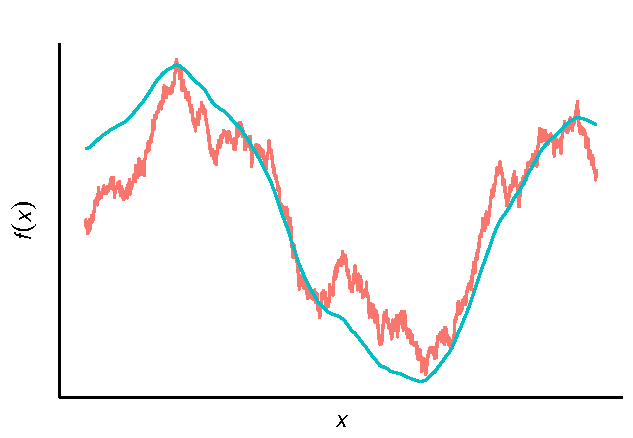
\includegraphics[width=0.7\textwidth]{figure/02-conv_in_norm}
%  \caption[Pointwise closeness does not imply closeness in norm.]{In a RKHS, two functions which are close together in norm are close pointwise, but the converse is not necessarily true. Functions which appear to be close to each other may actually diverge with respect to the norm of the RKHS.}
%\end{figure}

%The continuity condition also represents the weakest condition required for both the existence of an inner product and the evaluation of every function in $\cF$ at every point in the domain $\cX$.
While the continuity condition by definition is what makes an RKHS, it is neither easy to check this condition in practice, nor is it intuitive as to the meaning of its name.
In fact, there isn't even any mention of what a reproducing kernel actually is.
In order to benefit from the desirable continuity property of RKHS, we should look at this from another, more intuitive, perspective. 
By invoking the Riesz representation theorem, we see that for all $x\in\cX$, there exists a unique element $h_x\in\cF$ such that
\[
  f(x) = \delta_x(f) = \ip{f,h_x}_\cF, \forall f \in \cF
\]
holds. 
Since $h_x$ itself is a function in $\cF$, it holds that for every $x' \in \cX$ there exists a $h_{x'}\in\cF$ such that
\[
  h_{x}(x') = \delta_{x'}(h_{x}) = \ip{h_x,h_{x'}}_\cF.
\]
This leads us to the definition of a \emph{reproducing kernel} of an RKHS---the very notion that inspires its name.

\begin{definition}[Reproducing kernels]\label{def:repkern}
  Let $\mathcal F$ be a Hilbert space of functions over a non-empty set $\mathcal X$. 
  A symmetric, bivariate function $h:\mathcal X\times\mathcal X\rightarrow\mathbb R$ is called a \emph{kernel}, and it is a \emph{reproducing kernel} of $\mathcal F$ if $h$ satisfies
  \begin{itemize}
    \item $\forall x \in \mathcal X,\, h(\cdot, x) \in \mathcal F$; and
    \item $\forall x \in \mathcal X, \, f \in \mathcal F, \, \langle f, h(\cdot, x) \rangle_{\mathcal F} = f(x)$ (the reproducing property).
  \end{itemize}
  In particular, for any $x, x' \in \mathcal X$,
  \[
  	h(x,x') = \langle h(\cdot, x), h(\cdot, x') \rangle_{\mathcal F}.
  \]
\end{definition}

An important property for reproducing kernels of a RKHS is that they are positive-definite functions.
That is, $\forall a_1, \dots, a_n \in \mathbb R$ and $\forall x_1, \dots, x_n \in \mathcal X$,
\[
  \sum_{i=1}^n\sum_{j=1}^n a_i a_j h(x_i, x_j) \geq 0.
\]

\begin{proposition}[Reproducing kernels of RKHS are positive-definite]\label{thm:posdef}
  Let $\hXXR$ be a reproducing kernel for a Hilbert space $\cF$.
  Then $h$ is a symmetric and positive definite function.
\end{proposition}

\begin{proof}
  \begin{align*}
    \sum_{i=1}^n\sum_{j=1}^n a_i a_j h(x_i, x_j)	
    &= \sum_{i=1}^n\sum_{j=1}^n a_i a_j \langle  h(\cdot, x_i), h(\cdot, x_j) \rangle_{\mathcal F} \displaybreak[1] \\
    &= \Bigg\langle \sum_{i=1}^n a_i h(\cdot, x_i), \sum_{j=1}^n a_j h(\cdot, x_j) \Bigg\rangle_{\mathcal F} \\
    &= \Bigg\Vert \sum_{i=1}^n a_i h(\cdot, x_i) \Bigg\Vert_{\mathcal F}^2 \\
    & \geq 0 \qedhere
  \end{align*}
\end{proof}

\begin{remark}
  In the kernel method literature, a \emph{kernel} $\hXXR$ is usually defined as the inner product between inputs in feature space.
  That is, take $\phi:\cX\to\cV$, $x\mapsto\phi(x)$, where $\cV$ is a Hilbert space.
  Then the kernel is defined as $h(x,x') = \ip{\phi(x),\phi(x')}_\cV$, for any $x,x'\in\cX$.
  The space $\cV$ is known as the \emph{feature space} and the mapping $\phi$ the \emph{feature map}.
  In many mathematical models involving feature space mappings, elucidation of the feature map and feature space is not necessary, and thus computation  is made simpler by the use of kernels (known as the \emph{kernel trick}---\cite{hofmann2008kernel}).
  Note that kernels defined in this manner are positive definite, while in this thesis, we opt for a more general definition allowing kernels to not necessarily be positive.
  The relevance of this generality will be appreciated when we discuss reproducing kernel Kreĭn spaces in \cref{sec:rkkstheory}.
\end{remark}

Introducing the following definition of the \emph{kernel matrix} (also known as the \emph{Gram matrix}) is useful at this point.
\begin{definition}[Kernel matrix]
  Let $\{x_1,\dots,x_n\}$ be a sample of points, where each $x_i\in\cX$, and $h$ a kernel over $\cX$.
  Define the \emph{kernel matrix} $\bH$ for $h$ as the $n \times n$ matrix with $(i,j)$ entries equal to $h(x_i,x_j)$.
\end{definition}
Obviously, $\bH$ is a positive-definite matrix if the kernel that defines it is positive-definite: $\ba^\top\bH\ba = \sum_{i=1}^n\sum_{j=1}^n a_ia_jh(x_i,x_j) \geq 0$ for any choice of $a_1,\dots,a_n\in\bbR$ and $x_1,\dots,x_n\in\cX$.

So far, we have seen that reproducing kernels of a RKHS are positive-definite functions, and that RKHSs are Hilbert spaces with continuous evaluation functionals, but one might wonder what exactly the relationship between a reproducing kernel and a RKHS is.
%there are several questions we might like the answer to: What is the relationship between a reproducing kernel and an RKHS? Can we speak to its existence and uniqueness? What other properties does it have?
We assert the following:
\begin{itemize}
  \item For every RKHS $\cF$ of functions over a set $\cX$, there corresponds a unique, positive-definite reproducing kernel $\hXXR$, and vice-versa. That is, a Hilbert space is a RKHS if it possesses a unique, reproducing kernel.
  \item For every positive-definite function $\hXXR$, there corresponds a unique RKHS $\cF$ that has $h$ as its reproducing kernel.
\end{itemize}
Pictorially, the following relationships are established:

\tikzstyle{block} = [rectangle, draw, text width=6em, text centered, rounded corners, minimum height=4em]
\tikzstyle{singlearrow} = [draw,-implies,double distance=4pt, shorten >=0.5cm, shorten <=0.5cm]
\tikzstyle{doublearrow} = [draw,implies-implies,double distance=4pt, shorten >=0.5cm, shorten <=0.5cm]

\vspace{0.5em}
\begin{figure}[H]
  \centering
  \begin{tikzpicture}[node distance=1cm, auto]
    \node (init) {};
    \node [block] (repkern) {Reproducing kernels};
    \node [block, below=1cm of repkern, xshift=-3cm] (pd) {P.d. functions};
    \node [block, below=1cm of repkern, xshift=3cm] (rkhs) {RKHS};    
    
    \path [singlearrow] (pd) -- node [text width=2.5cm,midway,above,align=center,yshift=0.2cm] {\cref{thm:moorea}} (rkhs);
    \path [doublearrow] (repkern.east) -- node [text width=2.5cm,midway,above,align=left,xshift=1.5cm] {\cref{thm:rkhsunique}} (rkhs.north);
    \path [doublearrow] (repkern.west) -- node [text width=2.5cm,midway,above,align=right,xshift=-1.5cm] {\cref{thm:posdef}} (pd.north);
  \end{tikzpicture}  
  \caption[Relationship between p.d. functions, rep. kernels, and RKHSs]{Relationships between positive definite functions, reproducing kernels, and RKHSs.}
\end{figure}
\vspace{-0.5em}

In essence, the notion of positive-definite functions and reproducing kernels of RKHSs are equivalent, and that there is a bijection between the set of positive-definite kernels and the set of RKHSs.
The rest of this section is a consideration of these assertions, addressed by the two theorems that follow.

\begin{theorem}[RKHS uniqueness]\label{thm:rkhsunique}
  Let $\cF$ be a Hilbert space of functions over $\cX$.
  $\cF$ is a RKHS if and only if $\cF$ has a reproducing kernel $\hXXR$, and that $h$ is unique to $\cF$.
\end{theorem}

\begin{proof}
  First we tackle existence, i.e., we prove that $\cF$ is a RKHS if and only if $\cF$ has a reproducing kernel.
  Suppose $\cF$ is a Hilbert space of functions, and $\hXXR$ is a reproducing kernel for $\cF$.
  Then, choosing $\delta=\epsilon / \norm{h(\cdot,x)}_\cF$, for any $f \in \cF$ such that $\norm{f-g}_\cF < \delta$, we have
  \begin{align*}
    \vert \delta_x (f) - \delta_x (g) \vert 
    &= \vert (f-g)(x) \vert \\
    &= |\ip{f-g,h(\cdot,x)}_\cF| \mycomment{(reproducing property)} \\
    &\leq \norm{h(\cdot,x)}_\cF \, \norm{f-g}_\cF \mycomment{(Cauchy-Schwarz)} \\
    &= \epsilon.
  \end{align*}
  Thus, the evaluation functional is (uniformly) continuous on $\cF$, and by definition, $\cF$ is a RKHS.
  Now suppose that $\cF$ is a RKHS, and $h$ is a kernel function over $\cX\times\cX$.
  The reproducing property of $h$ is had by following the argument preceding \cref{def:repkern}.
 
  As for uniqueness, assume that the RKHS $\cF$ has two reproducing kernels $h_1$ and $h_2$. 
  Then, $\forall f\in\cF$ and $\forall x\in\cX$,
  \begin{align*}
    \ip{f,h_1(\cdot,x) - h_2(\cdot,x)}_\cF = f(x) - f(x) = 0.
  \end{align*}
  In particular, if we take $f = h_1(\cdot,x) - h_2(\cdot,x)$, we obtain $\norm{h_1(\cdot,x) - h_2(\cdot,x)}^2_\cF = 0$.
  Thus, $h_1=h_2$.
\end{proof}

\begin{theorem}[Moore-Aronszajn]\label{thm:moorea}
  If $\hXXR$ is a positive-definite function then there exists a unique RKHS whose reproducing kernel is $h$.
\end{theorem}

\begin{proof}[Sketch proof]
  Most of the details here have been omitted, except for the parts which we feel are revealing as to the properties of an RKHS.
  For a complete proof, see \citet{berlinet2011reproducing}. 
  Start with the linear space
  \[
    \cF_0 = \left\{ f_n:\cX\to\bbR \, \Big| \, f_n = \sum_{i=1}^n w_i h(\cdot,x_i), x_i\in\cX, w_i\in\bbR, n\in\bbN \right\}
  \]
  and endow this linear space with the following inner product:
  \[\label{eq:rkhsinnerprod}
    \left\langle \sum_{i=1}^n w_i h(\cdot,x_i), \sum_{j=1}^m w_j' h(\cdot,x_j') \right\rangle_{\cF_0} = \sum_{i=1}^n\sum_{j=1}^m w_i w_j' h(x_i,x_j').
  \]
  It may be shown that this indeed a valid inner-product satisfying the conditions laid in \cref{def:innerprod}.
  At this point, the reproducing property is already had:   \begin{align*}
    \big\langle f_n, h(\cdot,x) \big\rangle_{\cF_0} 
    &= \left\langle \sum_{i=1}^n w_i h(\cdot,x_i), h(\cdot,x) \right\rangle_{\cF_0} \\
    &= \sum_{i=1}^n w_i h(x_i,x) \\
    &= f_n(x),
  \end{align*}
  for any $f_n\in\cF_0$.
  
  Let $\cF$ be the completion of $\cF_0$ with respect to this inner product.
  In other words, define $\cF$ to be the set of functions $f:\cX\to\bbR$ for which there exists a Cauchy sequence $\{f_n\}_{n=1}^\infty$ in $\cF_0$ converging pointwise to $f \in \cF$.
  The inner product for $\cF$ is defined to be
  \[
    \ip{f,f'}_\cF = \lim_{n\to\infty} \ip{f_n,f_n'}_{\cF_0}.
  \]
  The sequence $\{ \ip{f_n,f_n'}_{\cF_0} \}_{n=1}^\infty$ is convergent and does not depend on the sequence chosen, but only on the limits $f$ and $f'$ \citep[Lemma 5]{berlinet2011reproducing}.
  We may check that this indeeds defines a valid inner product.
  The reproducing property carries over to the completion:
  \begin{align*}
    \ip{f,h(\cdot,x)}_\cF 
    &= \lim_{n\to\infty} \ip{f_n,h(\cdot,x)}_{\cF_0} \\
    &= \lim_{n\to\infty} f_n(x) \\
    &= f(x).
  \end{align*}
  
  To prove uniqueness, let $\cG$ be another RKHS with reproducing kernel $h$.
  $\cF$ has to be a closed subspace of $\cG$, since $h(\cdot,x) \in \cG$ for all $x\in\cX$, and because $\cG$ is complete and contains $\cF_0$ and hence its completion.
  Using the orthogonal decomposition theorem, we have $\cG = \cF \oplus \cF^\bot$, i.e. any $g\in\cG$ can be decomposed as $g = f + f^c$, $f\in\cF$ and $f^c\in\cF^\bot$.
  For each element $g\in\cG$ we have that, for all $x\in\cX$,
  \begin{align*}
    g(x) &= \ip{g,h(\cdot,x)}_\cG \\
    &= \big\langle f+f^c, h(\cdot,x) \big\rangle_\cG \\
    &= \big\langle f, h(\cdot,x) \big\rangle_\cG + \cancelto{0}{\big\langle f^c, h(\cdot,x) \big\rangle_\cG} \\
    &= f(x)
  \end{align*}
  so therefore $g\in\cF$ too.
  It must be that $\cF\equiv\cG$.
  %$\cF\cong\cG$.
%  
%  Minor detail: $f^c \in \cF^\bot \Rightarrow f^c \in \{f\in\cF | \ip{f,f'} = 0 \ \forall f'\in\cF \}$. Thus
%  \begin{align*}
%    \big\langle f^c, h(\cdot,x) \big\rangle_\cG 
%    &= f^c(x) \\
%    &= \big\langle f^c, h(\cdot,x) \big\rangle_\cF \\
%    &= 0
%  \end{align*}
%  It is evident that the inner product as defined is symmetric, linear, and positive-definite due to the positive-definiteness of reproducing kernels.
%  The only non-trivial condition to check is that whether $\ip{f_n,f_n}_{\cF_0}$ implies $f_n=0$.
%  To see this, realise that
%  \begin{align*}
%    0 &\leq 
%    1
%  \end{align*}
%  
%  By the Cauchy-Schwarz inequality, we see that
%  \begin{align*}
%    |f_n(x)| &= \big| \big\langle f_n, h(\cdot,x) \big\rangle_{\cF_0} \big| \\
%    &\leq \Vert h(\cdot,x) \Vert_{\cF_0} \cdot \Vert f_n \Vert_{\cF_0}    \\
%    &= \sqrt{h(x,x)} \cdot \Vert f_n \Vert_{\cF_0}
%  \end{align*}
%  so convergence in norm implies pointwise convergence.
%  By a similar argument in the proof of \cref{thm:normpointconv}, we also get that pointwise convergence is implied by convergence in norm for this space.
%  In particular, for every Cauchy sequence $\{f_n\}_{n=1}^\infty$ in $\cF_0$, $\big\{f_n(x)\big\}_{n=1}^\infty$ is a Cauchy sequence on the real line.
%  Complete the space $\cF_0$ by adjoining all of these limits to it, and call this completed space $\cF$.
%  
%  Furthermore, note that $\big\vert \norm{f_n}_{\cF_0} - \norm{f_m}_{\cF_0} \big\vert \leq \norm{f_n - f_m}_{\cF_0}$ (triangle inequality), so for a Cauchy sequence $\{f_n\}_{n=1}^\infty$ in a complete space, $\norm{f_n}_{\cF_0}$ has a limit.
%  Define the norm of $\cF$ to be $\norm{f}_\cF = \lim_{n\to\infty} \norm{f_n}_{\cF_0}$ for any $f\in\cF$.
%  Next, extend the inner product from $\cF_0$ to $\cF$ by defining $\ip{f,g}_\cF = \lim_{n\to\infty} \langle f_n,g_n \rangle_{\cF_0}$, where
%  \[
%    \lim_{n\to\infty} \langle f_n,g_n \rangle_{\cF_0} = \lim_{n\to\infty} \half\left( \norm{f+g}_{\cF_0}^2 - \norm{f}_{\cF_0}^2 - \norm{g}_{\cF_0}^2\right).
%  \]
%  One can indeed verify this is a well-defined inner product.
\end{proof}

A consequence of the above proof is that we can show that any function $f$ in a RKHS $\mathcal F$ with kernel $h$ can be written in the form $f(x) = \sum_{i=1}^n h(x, x_i)w_i$, with some $(w_1,\dots,w_n)\in\bbR^n$, $n \in \mathbb N$. 
More precisely, $\mathcal F$ is the completion of the space $\mathcal G = \text{span}\{h(\cdot,x) \, | \, x \in \mathcal X \}$ endowed with the inner product as stated in \cref{eq:rkhsinnerprod}.





\section{Reproducing kernel Kreĭn space theory}\label{sec:rkkstheory}
%To state the obvious, multiplication of a kernel by a negative scalar results in a negative definite function.
%Such actions arise when building new function spaces from existing ones, such as via a polynomial-type or ANOVA-type construction, as we will see later in \cref{sec:constructrkks}.
%Do we forfeit all the nice properties of RKHS?
%As it turns out no, for the most relevant parts anyway.
In this section, we shall review basic Kreĭn and reproducing kernel Kreĭn space theory, and comment on the similarity and differences between it and RKHS.
Kreĭn spaces are spaces endowed with a Hilbertian topology, characterised by an inner product which is non-positive.
%To quote \citet{ong2004learning}, Kreĭn spaces are inner product spaces endowed with a Hilbertian topology, yet their inner product is no longer positive. 

\begin{definition}[Negative and indefinite inner products]
  Let $\ip{\cdot,\cdot}_\cF$ be an inner product of a vector space $\cF$, as per \cref{def:innerprod}.
  An inner product is said to be \emph{negative-definite} if for all $f\in\cF$, $\ip{f,f}_\cF \leq 0$.
  It is \emph{indefinite} if it is neither positive- nor negative-definite.
\end{definition}

\begin{definition}[Kreĭn space]
  An inner product space $\big(\cF,\ip{\cdot,\cdot}_\cF\big)$ is a \emph{Krein space} if there exists two Hilbert spaces $\big(\cF_+,\ip{\cdot,\cdot}_{\cF_+}\big)$ and $\big(\cF_-,\ip{\cdot,\cdot}_{\cF_-}\big)$ spanning $\cF$ such that
  \begin{itemize}
    \item All $f\in\cF$ can be decomposed into $f = f_+ + f_-$, where $f_+\in\cF_+$ and $f_- \in \cF_-$.
    \item This decomposition is orthogonal, i.e. $\cF_+ \cup \cF_- = \{0\}$, and $\ip{f_+,f_-}_\cF=0$ for all $f_+\in\cF_+$ and $f_-\in\cF_-$, with the inner product on $\cF$ defined below.
    \item $\forall f,f'\in\cF$, $\ip{f,f'}_\cF = \ip{f_+,f_+'}_{\cF_+}- \ip{f_-,f_-'}_{\cF_-}$.
  \end{itemize}
\end{definition}

Let $P$ be the projection of the Kreĭn space $\cF$ onto $\cF_+$, and $Q=I-P$ the projection onto $\cF_-$.
These are caleld the \emph{fundamental projections} of $\cF$.
We shall refer to $\cF_+$ as the \emph{positive subspace}, and $\cF_-$ as the \emph{negative subspace}.
These monikers stem from the fact that for all $f,f' \in \cF$, $\ip{Pf,Pf'}_{\cF_+} \geq 0$ while $\ip{Qf,Qf'}_{\cF_-} \leq 0$.
We introduce the notation $\ominus$ to refer to the Kreĭn space decomposition: $\cF = \cF_+ \ominus \cF_-$.
There is then a notion of an \emph{associated Hilbert space}.

\begin{definition}[Associated Hilbert space]
  Let $\cF$ be a Kreĭn space with decomposition into Hilbert spaces $\cF_+$ and $\cF_-$.
  Denote by $\cF_\cH$ the associated Hilbert space defined by $\cF_\cH = \cF_+ \oplus \cF_-$, with inner product 
  \[
    \ip{f,f'}_{\cF_\cH} = \ip{f_+,f_+'}_{\cF_+} + \ip{f_-,f_-'}_{\cF_-},
  \]
  for all $f,f'\in\cF$.
%  Likewise,
%  \[
%    \cF = \cF_+ \ominus \cF_-,
%  \]
%  and hence $\ip{f,f'}_{\cF} = \ip{f_+,f_+'}_{\cF_+} - \ip{f_-,f_-'}_{\cF_-}$.
\end{definition}

The associated Hilbert space can be found via the linear operator $J = P - Q$ called the \emph{fundamental symmetry}.
%, which satisfies $J = J^{-1} = J^\top$.
That is, a Kreĭn space $\cF$ can be turned into its associated Hilbert space by using the positive-definite inner product of the associated Hilbert space as $\ip{f,f'}_{\cF_\cH} = \ip{f,Jf'}_\cF$, for all $f,f'\in\cF$.
The converse is true too: Starting from a Hilbert space $\cF_\cH$ and an operator $J$, the vector space endowed with the inner product $\ip{f,f'}_\cF = \ip{f,Jf'}_{\cF_\cH}$, for all $f,f'\in\cF$, is a Kreĭn space.

We realise that for a Kreĭn space $\cF$, $|\ip{f,f}_\cF| \leq \norm{f}^2_{\cF_\cH}|$ for all $f\in\cF$, and we say that $\cF_\cH$ majorises the $\cF$, and in fact it is the smallest Hilbert space to do so.
The strong topology on $\cF$ is defined to be the topology arising from the norm of $\cF_\cH$, and this does not depend on the decomposition chosen \citep{ong2004learning}.

\begin{definition}[Reproducing kernel Krein space]
  A Krein space $\cF$ of real-valued functions $f:\mathcal X \rightarrow \mathbb R$ on a non-empty set $\mathcal X$ is called a \emph{reproducing kernel Krein space} if the evaluation functional $\delta_x: f \mapsto f(x)$ is continuous on $\cF$, $\forall x \in \cX$, endowed with its strong topology (i.e. the topology of its associated Hilbert space $\cF_\cH$).
\end{definition}

One might wonder whether the uniqueness theorem (\cref{thm:rkhsunique}) holds for RKKS.
Indeed, for every RKKS $\cF$ of functions over a set $\cX$, there corresponds a unique reproducing kernel $\hXXR$.

\begin{lemma}[Uniqueness of kernel for RKKS]
  Let $\cF$ be a RKKS of functions over a set $\cX$, with $\cF = \cF_+ \ominus \cF_-$.
  Then, $\cF_+$ and $\cF_-$ are both RKHS with kernel $h_+$ and $h_-$, and the kernel $h = h_+ - h_-$ is a unique, symmetric, reproducing kernel for $\cF$.  
\end{lemma}

\begin{proof}
  Since $\cF$ is a RKKS, evaluation functionals are continuous on $\cF$ with respect to topology of the associated Hilbert space $\cF_\cH = \cF_+ \oplus \cF_-$.
  Therefore, $\cF_\cH$ is a RKHS, and so too are $\cF_+$ and $\cF_-$ with respective kernels $h_+$ and $h_-$.
  
  Furthermore, $h(\cdot,x) \in\cF$ since $h_+(\cdot,x) \in\cF_+$ and $h_-(\cdot,x) \in\cF_-$ for some $x\in\cX$.
  Then, for any $f\in\cF$,
  \begin{align*}
    \ip{f, h(\cdot,x)}_\cF 
    &= \ip{f, h_+(\cdot,x)}_{\cF} - \ip{f, h_-(\cdot,x)}_{\cF} \\ 
    &= \ip{f_+, h_+(\cdot,x)}_{\cF_+} - \cancelto{0}{\ip{f_-, h_+(\cdot,x)}_{\cF_-}} \\
    &\phantom{==} - \cancelto{0}{\ip{f_+, h_-(\cdot,x)}_{\cF_+}} + \ip{f_-, h_-(\cdot,x)}_{\cF_-} \\
    &= f_+(x) + f_-(x) \\
    &= f(x)
  \end{align*}
  The last two lines are achieved by linearity of evaluation functionals ($\delta_x(f_+) + \delta_x(f_-) = \delta_x(f_+ + f_-)$), and the fact that $f = f_+ + f_-$ (by the Kreĭn space decomposition).
  We have that $h=h_+ - h_-$ is a reproducing kernel for $\cF$.
  Uniqueness follows as a consequence of the non-degeneracy condition of the respective inner products for $\cF_+$ and $\cF_-$.
\end{proof}

\begin{remark}
  Unlike reproducing kernels of RKHSs, reproducing kernels of RKKSs may not be positive-definite.
%  As we said earlier, difference in kernels may not be positive-definite and therefore not kernels in the truest sense of the word.
%  Rather, they should be referred to as \emph{generalised kernels}, as they are defined in the vector space generated out of the cone of positive kernels. 
%  Regardless, we shall keep referring to them as kernels for brevity.
\end{remark}

The analogue of the Moore-Aronszajn theorem holds partially for RKKS, up to uniqueness.
That is, there is \emph{at least} one associated RKKS with kernel $\hXXR$ if and only if $h$ can be decomposed as the difference between two positive kernels $h_+$ and $h_-$ over $\cX$, i.e., $h=h_+-h_-$.
The proof of this statement is rather involved, so is omitted in the interest of maintaining coherence to the discussion at hand.
This subject has been studied by various authors, one may refer to works by \citet[Theorem 2 \& Example in Section 4]{alpay1991some}, and \citet[Theorem 2.28]{mary2003hilbertian}.
%\begin{lemma}[Non-uniqueness of RKKS for kernel]
%  Let $h$ be a kernel over $\cX$.
%  There is (at least) one associated RKKS with kernel $h$ if and only if $h$ can be decomposed as the difference between two positive kernels $h_+$ and $h_-$ over $\cX$, i.e., $h=h_+-h_-$.
%\end{lemma}
%
%\begin{proof}
%  The existence and (non-)uniqueness of a RKKS associated with a kernel $h$ relies on the ability to complete the span of $h(\cdot,x)$, much like in the proof of the Moore-Aronszajn theorem.
%  As it turns out, this is rather involved, so is omitted in the interest of maintaining coherence to the discussion at hand.
%  This subject has been studied by various authors, one may refer to a proof of this lemma in works by \citet[Theorem 2 \& Example in Section 4]{alpay1991some}, and \citet[Theorem 2.28]{mary2003hilbertian}.
%\end{proof}

The take-away message as we close this section is that there is no bijection, but a surjection, between the set of RKKS and the set of bivariate, symmetric functions over $\cX\times\cX$.
In any case, Hilbertian topology applies to Kreĭn spaces via the associated Hilbert space, and in particular, RKKS provide a functional space for which evaluation functionals are continuous.
The motivation for the use of Kreĭn spaces will become clear when constructing function spaces out of (scaled) building block RKHS later in \cref{sec:constructrkks}.


\section{RKHS building blocks}\label{sec:rkhsbuild}
This section describes what we refer to as the ``building block'' RKHSs of functions.
In the context of regression modelling using I-priors, we may assume that the regression function lies in any one of these single RKHSs, although it may be more appropriate to consider function spaces built upon these RKHSs for more complex models.
Construction of new function spaces from these building block RKHSs will be discussed in the next section.

\subsection{The RKHS of constant functions}

The vector space of constant functions $\cF$ over a set $\cX$ contains the functions $f:\cX \to \bbR$ such that $f(x) = c_f \in \bbR$, $\forall x \in \cX$.
These functions would be useful to model an overall average, i.e. an ``intercept effect''.
The space $\cF$ can be equipped with a norm to form an RKHS, as shown in the following proposition.

\begin{proposition}[RKHS of constant functions]
  The space $\cF$ as described above endowed with the norm $\norm{f}_\cF = \vert c_f \vert$ forms an RKHS with the reproducing kernel $h:\cX\times\cX\to\bbR$ as defined, rather simply, by
  \[
    h(x,x') = 1,
  \]
  known as the constant kernel.
\end{proposition}

\begin{proof}
  If $\cF$ is an RKHS with kernel $h$ as described, then $\cF$ is spanned by the  functions $h(\cdot,x) = 1$, so it is clear that $\cF$ consists of constant functions over $\cX$.
  On the other hand, if the space $\cF$ is equipped with the inner product $\ip{f,f'}_\cF = c_f c_{f'}$, then the reproducing property follows, since $\ip{f,h(\cdot,x)}_\cF = c_f = f(x)$.
  Hence, $\norm{f}_\cF = \sqrt{\ip{f,f}_\cF} = \vert c_f \vert$.
\end{proof}

\begin{remark}
  In I-prior modelling, it is simpler to consider the intercept of a regression model as a parameter to be estimated, rather than a separate function within an RKHS of constant functions for which its posterior is to be estimated.
  See \cref{sec:intercept} in \cref{chapter4} for further details.  
\end{remark}

\begin{figure}[hbt]
  \centering
  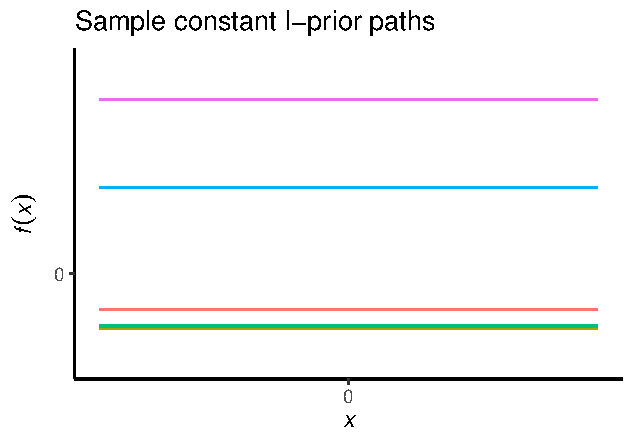
\includegraphics[width=0.54\textwidth]{figure/02-kernel_path_const}
  \caption{Sample I-prior paths from the RKHS of constant functions.}
\end{figure}

\subsection{The canonical (linear) RKHS}

Consider a function space $\cF$ over $\cX$ which consists of functions of the form $f_\beta:\cX\to\bbR$, $f_\beta: x \mapsto \ip{x,\beta}_\cX$ for some $\beta\in\bbR$.
Suppose that $\cX \equiv \bbR^p$, then $\cF$ consists of the linear functions $f_\beta(x) = x^\top\beta$.
More generally, if $\cX$ is a Hilbert space, then its continuous dual consists of elements of the form $f_\beta = \ip{\cdot,\beta}_\cX$ by the Riesz representation theorem.
We can show that the continuous dual space of $\cX$ is a RKHS which consists of these linear functions.

\begin{proposition}[The canonical RKHS]
  The continuous dual space a Hilbert space $\cX$, denoted by $\cX^*$, is a RKHS of linear functions over $\cX$ of the form $\ip{\cdot,\beta}_\cX$, $\beta\in\cX$. Its reproducing kernel $h:\cX\times\cX\to\bbR$ is defined by
  \[
    h(x,x') = \ip{x,x'}_{\cX}.
  \]
\end{proposition}

\begin{proof}
  Define $f_\beta := \ip{\cdot,\beta}_\cX$ for some $\beta \in \cX$.
  Clearly this is linear and continuous, so $f_\beta\in\cX^*$, and so $\cX^*$ is a Hilbert space containing functions $f:\cX\to\bbR$ of the form $f_\beta(x) = \ip{x,\beta}_\cX$.
  By the Riesz representation theorem, every element of $\cX^*$ has the form $f_\beta$.
  It also gives us a natural isometric isomorphism such that the following is true:
  \[
    \ip{\beta,\beta'}_\cX = \ip{f_\beta,f_{\beta'}}_{\cX^*}.
  \]
  Hence, for any $f_\beta\in\cX^*$, 
  \vspace{-0.5em}
  \begin{align*}
    f_\beta(x) 
    &= \ip{x,\beta}_\cX \\
    &= \ip{f_x,f_{\beta}}_{\cX^*} \\
    &= \big\langle \ip{\cdot,x}_\cX,f_{\beta} \big\rangle_{\cX^*}. \vspace{-0.5em}
  \end{align*}
  Thus, $h:\cX\times\cX\to\bbR$ as defined by $h(x,x') = \ip{x,x'}_\cX$ is the reproducing kernel of $\cX^*$.
\end{proof}

In many other literature, the kernel $h(x,x') = \ip{x,x'}_\cX$ is also known as the \emph{linear kernel}.
The use of the term `canonical' is fitting not just due to the relation between a Hilbert space and its continuous dual space.
Let $\phi:\cX\to\cV$ be the feature map from the space of covariates (inputs) to some feature space $\cV$.
Suppose both $\cX$ and $\cV$ are Hilbert spaces, then a kernel is defined as 
\[
  h(x,x') = \ip{\phi(x),\phi(x')}_\cV.
\]
Taking the feature map to be $\phi(x) = \ip{\cdot,x}_\cX$, we can prove the reproducing property to obtain $h(x,x') = \ip{x,x'}_\cX$, which implies $\phi(x) = h(\cdot,x)$, and thus $\phi$ is the \emph{canonical feature map} \citep[Lemma 4.19]{steinwart2008support}.

\begin{figure}[H]
  \centering
  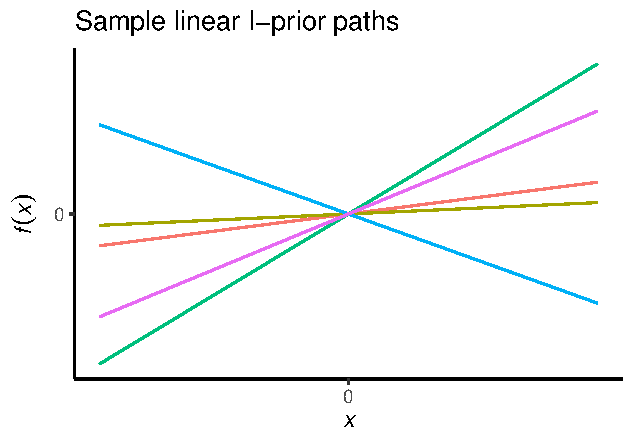
\includegraphics[width=0.53\textwidth]{figure/02-kernel_path_canonical}
  \caption{Sample paths from the canonical RKHS.}
\end{figure}

The origin of a Hilbert space may be arbitrary, in which case a centring may be appropriate.
We define the centred canonical RKHS as follows.

\begin{definition}[Centred canonical RKHS]
  Let $\cX$ be a Hilbert space, $\Prob$ be a probability measure over $\cX$, and $\mu\in\cX$ be the mean of a random element $X\in\cX$. 
%  (i.e. $\E\ip{x,x'}_{\cX}  = \ip{\mu,x'}_{\cX}$ for all $x' \in \cX$) with respect to this probability measure.
  Define $(\cX - \mu)'$, the continuous dual space of $\cX - \mu$, to be the \emph{centred canonical RKHS}.
  $(\cX - \mu)'$ consists of the centred linear functions $f_\beta(x)=\ip{x-\mu,\beta}_\cX$, for $\beta\in\cX$, such that $\E \big( f_\beta(X) \big) = 0$.
  The reproducing kernel of $(\cX - \mu)'$ is
  \[
    h(x,x') = \ip{x-\mu,x'-\mu}_\cX.
  \]
\end{definition}

That the centred canonical RKHS consists of zero mean function, $\E \big( f_\beta(X) \big)  = 0$, consider the following argument:
\vspace{-0.5em}
\begin{align*}
  \E \big( f_\beta(X) \big) 
  &= \E \ip{X-\mu,\beta}_\cX \\
  &= \E \ip{X,\beta}_\cX - \ip{\mu,\beta}_\cX, \vspace{-0.5em}
\end{align*}
and since $\E \ip{X,\beta}_\cX = \ip{\mu,\beta}_\cX$ for any $\beta\in\cX$, the results follows.

\begin{remark}\label{rem:empircent}
  In practice, the probability measure $\Prob$ over $\cX$ is unknown, so we find it useful to use the empirical distribution over $\cX$ instead, so that $\cX$ is centred by the sample mean $\hat\mu = \frac{1}{n}\sum_{i=1}^n x_i$.  
\end{remark}

\subsection{The fractional Brownian motion RKHS}

Brownian motion, which also goes by the name Wiener process, has been an inquisitive subject in the mathematical sciences, and here, we describe a function space motivated by a generalised version of Brownian motion paths.

Suppose $B_\gamma(t)$ is a continuous-time Gaussian process on $[0,T]$, i.e. for any finite set of indices $t_1,\dots,t_k$, where each $t_j \in [0,T]$, $\big(B_\gamma(t_1),\dots,B_\gamma(t_k)\big)$ is a multivariate normal random variable.
$B_\gamma(t)$ is said to be a \emph{fractional Brownian motion} (fBm) if $\E \big( B_\gamma(t)\big) = 0$ for all $t \in [0,T]$ and 
\vspace{-0.5em}
\[
  \Cov\big( B_\gamma(t),B_\gamma(s) \big) = \half\big( |t|^{2\gamma} + |s|^{2\gamma} - |t-s|^{2\gamma} \big) \hspace{1cm} \forall t,s \in [0,T],
\]
where $\gamma \in (0,1)$ is called the \emph{Hurst index}, \emph{Hurst parameter} or even \emph{Hurst coefficient}.
Introduced by \citet{mandelbrot1968fractional}, fBms are a generalisation of Brownian motion.
The Hurst parameter plays two roles: 1) it describes the raggedness of the resultant motion, with higher values leading to smoother motion; and 2) it determines the type of process the fBm is, as past increments of $B_\gamma(t)$ are weighted by $(t-s)^{\gamma-1/2}$.
When $\gamma=1/2$ exactly, the fBm is a standard Brownian motion and its increments are independent; when $\gamma > 1/2$ (resp. $\gamma < 1/2$) its increments are positively (resp. negatively) correlated.

Now, let $\cX$ be a Hilbert space. 
\citet[Theorem 3]{schoenberg1937} has shown that, for $0 < \gamma\leq 1$, there exists a Hilbert space $\cV$ and a function $\phi_\gamma:\cX\to\cV$ such that $\forall x,x' \in \cX$,
\[
  \big\Vert \phi_\gamma(x) - \phi_\gamma(x') \big\Vert_\cV = \norm{x-x'}_\cX^\gamma.
\]
Using the polarisation identity, 
%\begin{align*}
%  2\big\langle \phi_\gamma(x), \phi_\gamma(x') \big\rangle_\cV 
%  &= \big\Vert \phi_\gamma(x) \big\Vert_\cV^2 + \big\Vert \phi_\gamma(x') \big\Vert_\cV^2 - \big\Vert \phi_\gamma(x) - \phi_\gamma(x') \big\Vert_\cV^2  \\
%  &= \norm{x}_\cX^{2\gamma} + \norm{x'}_\cX^{2\gamma} - \norm{x-x'}_\cX^{2\gamma}
%\end{align*} 
we find that the kernel of the RKHS with feature space $\cV$ and feature map $\phi_\gamma$ defines a kernel function $h:\cX\times\cX\to\bbR$ identical to the fBm covariance kernel.

\begin{definition}[Fractional Brownian motion RKHS]\label{def:fbmrkhs}
  \hspace{-1.7pt}The fractional Brownian motion (fBm) RKHS $\cF$ is the space of functions on the Hilbert space $\cX$ possessing the reproducing kernel $h_\gamma:\cX\times\cX\to\bbR$ defined by
  \[
    h_\gamma(x,x') = \big\langle \phi_\gamma(x), \phi_\gamma(x') \big\rangle_\cV = \half\big( \norm{x}_\cX^{2\gamma} + \norm{x'}_\cX^{2\gamma} - \norm{x-x'}_\cX^{2\gamma} \big),
  \]
  which depends on the Hurst coefficient $\gamma \in (0,1)$.
  We shall reference this space as the fBm-$\gamma$ RKHS.
\end{definition}

\begin{remark}
  When $\gamma=1$, by the polarisation identity we get $h(x,x') = \ip{x,x'}_\cX$, which is the (reproducing) kernel of the canonical RKHS.
\end{remark}

From its construction, it is clear that the fBm kernel is positive definite, and thus defines an RKHS.
That the fBm RKHS describes a space of functions is proved in \citet{cohen2002}, who studied this space in depth. 
It is also noted in the collection of examples of \citet[pp.71 \& 319]{berlinet2011reproducing}.

The Hurst coefficient $\gamma$ controls the ``smoothness'' of the functions in the RKHS. 
We can talk about smoothness in the context of Hölder continuity of functions.

\begin{definition}[Hölder condition]
  A function $f$ over a set $(\cX, \norm{\cdot}_\cX)$ is said to be \emph{Hölder continuous} of order $0 <\gamma\leq 1$ if there exists a $C>0$ such that $\forall x,x'\in\cX$,
  \[
    \vert f(x) - f(x') \vert \leq C \norm{x-x'}^\gamma.
  \]
\end{definition}

Functions in the Hölder space $\text{C}^{k,\gamma}(\cX)$, where $k\geq 0$ is an integer, consists of those functions over $\cX$ having continuous derivatives up to order $k$ and such that the $k$th partial derivatives are Hölder continuous of order $\gamma$.
Unlike realisations of actual fBm paths with Hurst index $\gamma$, which are well-known to be almost surely Hölder continuous of order less than $\gamma$ \citep[Theorem 4.1.1]{embrechts2002selfsimilar}, functions in its namesake RKHS are strictly smoother.

%\begin{claim}
%  Let $\cF$ denote the fBm RKHS of functions over $\cX$ with Hurst parameter $\gamma \in (0,1)$, and the kernel $h$ as defined in  \cref{def:fbmrkhs}.
%  Then,
%  \begin{enumerate}[label=(\roman*)]
%    \item The functions in $\cF$ are Hölder continuous of order $\gamma$.  
%    \item The basis functions $h(\cdot,x)$ are Hölder continuous of order $2\gamma$.
%  \end{enumerate}
%\end{claim}

\begin{proposition}
  The fBm-$\gamma$ RKHS $\cF$ of functions over $(\cX, \norm{\cdot}_\cX)$ are Hölder continuous of order $\gamma$.
\end{proposition}

\begin{proof}
  For some $f \in \cF$ we have $f(x) = \ip{f,h(\cdot,x)}_\cF$ by the reproducing property of the kernel $h$ of $\cF$.
  It follows from the Cauchy-Schwarz inequality that for any $x,x'\in\cX$,
  \begin{align*}
    \vert f(x) - f(x') \vert 
    &= \vert \ip{f,h(\cdot,x) - h(\cdot,x')}_\cF \vert \\
    &\leq \norm{f}_\cF \, \big\Vert h(\cdot,x) - h(\cdot,x') \big\Vert_\cF \\
    &= \norm{f}_\cF \, \norm{x-x'}_\cX^{\gamma},
  \end{align*}
  since
  \begin{align*}
    \big\Vert h(\cdot,x) - h(\cdot,x') \big\Vert_\cF ^2
    &= \big\Vert h(\cdot,x) \big\Vert_\cF ^2 + \big\Vert h(\cdot,x') \big\Vert_\cF ^2 - 2 \ip{h(\cdot,x),h(\cdot,x')}_\cF \\
    &= h(x,x) + h(x',x') - 2 h(x,x') \\
    &= \norm{x-x'}_\cX^{2\gamma},
  \end{align*}  
  and thus proving the proposition.
\end{proof}
\pagebreak


\begin{figure}[hbt]
  \centering
  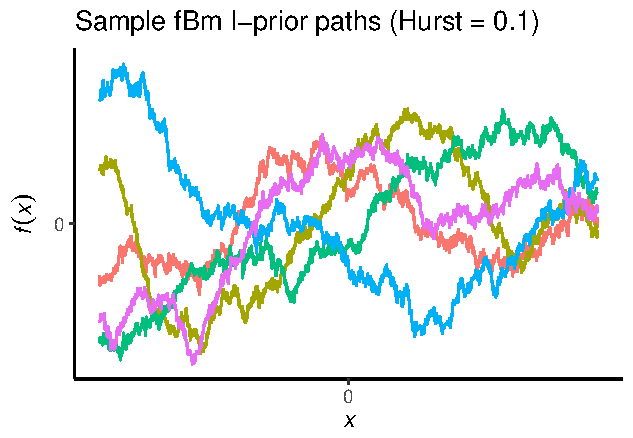
\includegraphics[width=0.49\textwidth]{figure/02-kernel_path_fbm_1}
  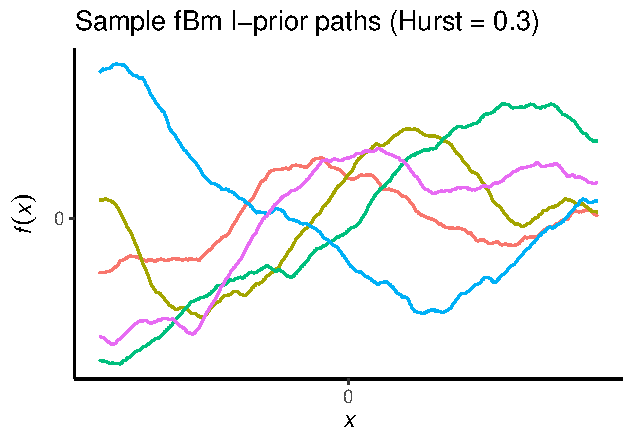
\includegraphics[width=0.49\textwidth]{figure/02-kernel_path_fbm_3}
  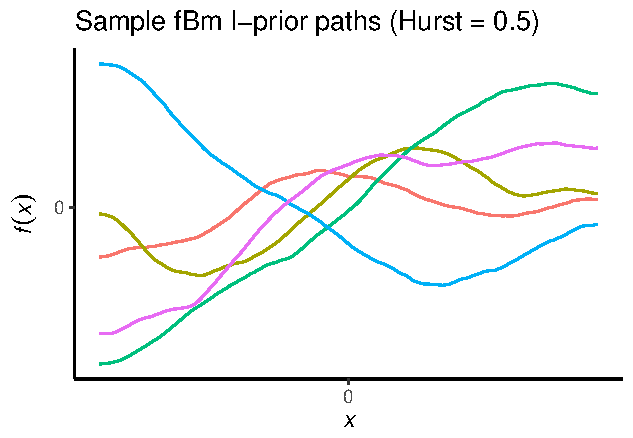
\includegraphics[width=0.49\textwidth]{figure/02-kernel_path_fbm_5}
  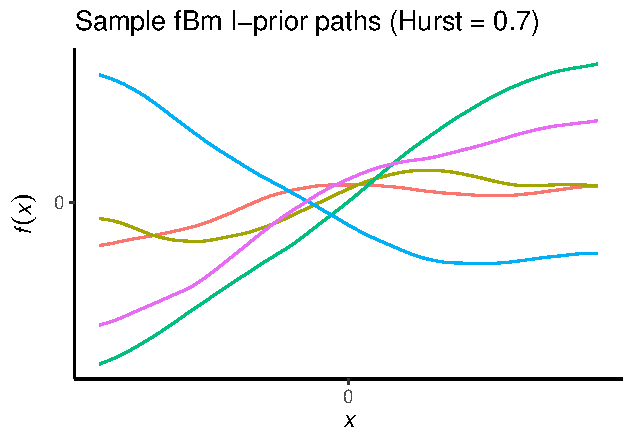
\includegraphics[width=0.49\textwidth]{figure/02-kernel_path_fbm_7}
  \caption[Sample I-prior paths from the fBm RKHS with varying Hurst coefficients.]{Sample I-prior paths from the fBm RKHS with varying Hurst coefficients. Note that the fBm-$\gamma$ RKHS contains functions that are rougher than these I-prior paths.}
\end{figure}

\vspace{-0.5em}
The fBm-$\gamma$ RKHS is spanned by the functions $h(\cdot,x)$, which means that $f(0)=0$ for all $f \in \cF$, which may be undesirable.
We define the centred fBm RKHS as follows.

\begin{definition}[Centred fBm RKHS]
  Let $\cX$ be a Hilbert space, $\Prob$ be a probability measure over $\cX$, and $\mu\in\cX$ be the mean 
%  (i.e. for a random element $X\in\cX$, $\E\ip{X,x'}_{\cX}  = \ip{\mu,x'}_{\cX}$ for all $x' \in \cX$) 
  with respect to this probability measure.
  The kernel $\bar h_\gamma:\cX\times\cX\to\bbR$ defined by
  \[
    \bar h_\gamma(x,x') = \half \E \left( \norm{x-X}_\cX^{2\gamma} + \norm{x'-X'}_\cX^{2\gamma} - \norm{x-x'}_\cX^{2\gamma} - \norm{X-X'}_\cX^{2\gamma} \right)
  \]
  is the reproducing kernel of the \emph{centred} fBm-$\gamma$ RKHS, which consists of functions $f$ in the fBm-$\gamma$ RKHS such that $\E \big( f(X) \big) = 0$.
  In the above definition, $X,X' \sim \Prob$ are two independent copies of a random vector $X \in \cX$.
\end{definition}

\begin{remark}
  Again, when $\gamma=1$, we get the reduction 
  \vspace{-0.1em}
  \begin{align*}
    \bar h_{\gamma=1}(x,x') 
    &= \half \E \left( \norm{x-X}_\cX^{2} + \norm{x'-X'}_\cX^{2} - \norm{x-x'}_\cX^{2} - \norm{X-X'}_\cX^{2} \right) \\
    &= \half \E \left( \ip{X,X}_\cX + \ip{X',X'}_\cX + 2\ip{x,x'}_\cX - 2\ip{x,X}_\cX - 2\ip{x',X'}_\cX\right) \\
    &= \ip{\mu,\mu}_\cX + \ip{x,x'}_\cX - \ip{x,\mu}_\cX - \ip{\mu,x'}_\cX \\
    &= \ip{x-\mu,x'-\mu}_\cX, \vspace{-1em}
  \end{align*}
  which is the (reproducing) kernel of the centred canonical RKHS.
\end{remark}

\begin{remark}
  For posterity, a general centring of any (positive-definite) kernel $\hXXR$ can be achieved via
  \[
    \bar h(x,x') = h(x,x') - \E\big(h(x,X')\big) - \E\big(h(X,x')\big) + \E\big(h(X,X')\big),
  \]  
  where expectations are taken for the random elements $X,X'\iid\Prob$, a probability measure over $\cX$.
  This centred kernel gives rise to the centred RKHS $\bar\cF$ of centred functions $\E\big(f(X)\big)$, $f\in\bar\cF$.
  As per \cref{rem:empircent}, the empirical distribution of $\Prob$ can be used to approximate the unknown, true $\Prob$.
\end{remark}

\subsection{The squared exponential RKHS}

The \gls*{SE} kernel function is indeed known to be the default kernel used for Gaussian process regression in machine learning.
It is a positive definite function, and hence defines an RKHS.
The definition of the SE RKHS is as follows.

\begin{definition}[Squared exponential RKHS]
  The squared exponential (SE) RKHS $\cF$ of functions over some set $\cX \subseteq \bbR^p$ equipped with the 2-norm $\norm{\cdot}_2$ is defined by the positive definite kernel $h_l:\cX\times\cX\to\bbR$ 
  \[
    h_l(x,x') = \exp\left( -\frac{\norm{x-x'}_2^2}{2l^2} \right).
  \]
  The real-valued parameter $l > 0$ is called the \emph{lengthscale} parameter, and is a smoothing parameter for the functions in the RKHS.
\end{definition}

It is known by many other names, including the Gaussian kernel, due to its semblance to the kernel of the Gaussian pdf. 
Especially in the machine learning literature, the term Gaussian radial basis functions (RBF) is used, and commonly the simpler parameterisation $\gamma = (2l^2)^{-1}$ is utilised.
\citet{duvenaud2014automatic} remarks that ``exponentiated quadratic'' is a more aptly descriptive name for this kernel.

Despite being used extensively for learning algorithms using kernels, an explicit study of the RKHS defined by the SE kernel was not done until recently by \citet{steinwart2006explicit}.
In that work, the authors describe the nature of real-valued functions in the SE RKHS by considering a a real restriction on the SE RKHS of functions over complex values.
Their derivation of an orthonormal basis of such an RKHS proved the SE kernel to be the reproducing kernel for the SE RKHS.

\begin{figure}[hbt]
  \centering
  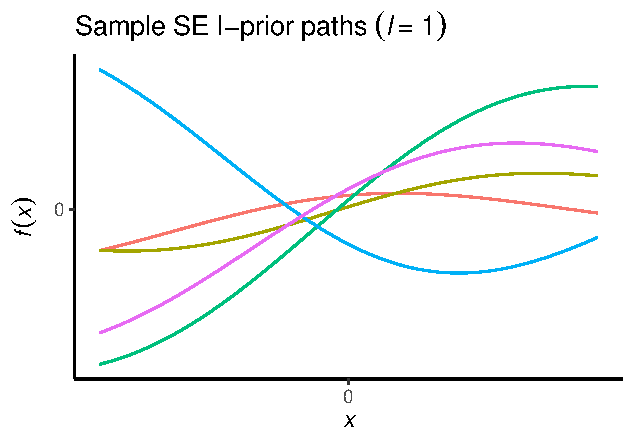
\includegraphics[width=0.49\textwidth]{figure/02-kernel_path_se_10}
  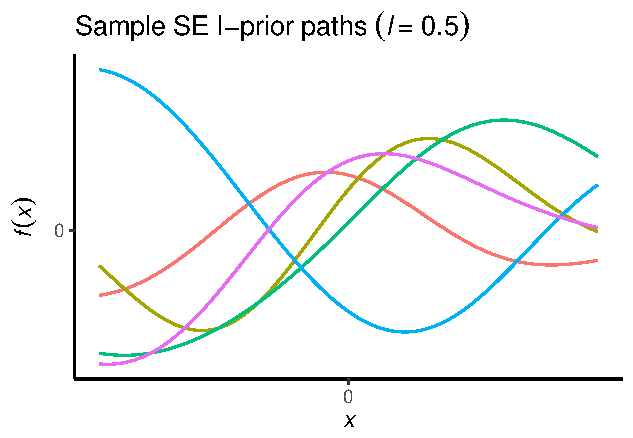
\includegraphics[width=0.49\textwidth]{figure/02-kernel_path_se_05}
  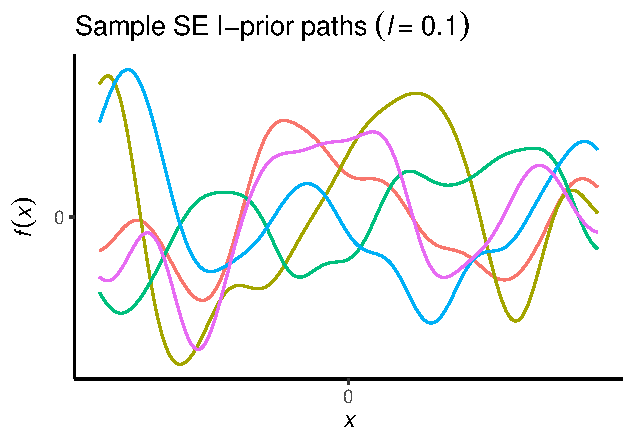
\includegraphics[width=0.49\textwidth]{figure/02-kernel_path_se_01}
  \caption{Sample paths from the SE RKHS with varying values for the lengthscale.}
\end{figure}

SE kernels are known to be ``universal''. That is, it satisfies the following definition of universal kernels due to \citet{micchelli2006universal}.

\begin{definition}[Universal kernel]
  Let $\text{C}(\cX)$ be the space of all continuous, complex-valued functions $f:\cX\to\bbC$ equipped with the maximum norm $\norm{\cdot}_\infty$, and denote $\cK(\cX)$ as the space of \emph{kernel sections} $ \overline{\text{span}}\{ h(\cdot,x) | x \in \cX \}$, where here, $h$ is a complex-valued kernel function.
  A kernel $h$ is said to be \emph{universal} if given any compact subset $\cZ \subset \cX$, any positive number $\epsilon$ and any function $f \in \text{C}(\cZ)$, there is a function $g \in \cK(\cZ)$ such that $\norm{f-g}_\cZ \leq \epsilon$.
\end{definition}

The consequence of this universal property vis-à-vis regression modelling is that any (continuous) regression function $f$ may be approximated very well by a function $\hat f$ belonging to the SE RKHS, and these two functions can get arbitrarily close to each other in the max norm sense.
This, together with the convenient computational advantages that the SE kernel brings \citep{raykar2007fast}, is a testament to the popularity of SE kernels.

In a similar manner to the two previous subsections, we may also derive the \emph{centred} SE RKHS. 

\begin{definition}[Centred SE RKHS]
  Let $\cX \subseteq \bbR^p$ be equipped with the 2-norm $\norm{\cdot}_2$, and let $\Prob$ denote the distribution over $\cX$.
  Assuming integrability of $h(x,X)$, for any $x\in\cX$ and a random element $X\in\cX$, the \emph{centred} squared exponential (SE) RKHS (with lengthscale $l$) of functions over $\cX$ is defined by the positive definite kernel $\hXXR$ 
  \[
    h(x,x') = e^{-\frac{\norm{x-x'}_2^2}{2l^2}} 
    - \E  e^{-\frac{\norm{x-X'}_2^2}{2l^2}} 
    - \E  e^{-\frac{\norm{X-x'}_2^2}{2l^2}} 
    + \E  e^{-\frac{\norm{X-X'}_2^2}{2l^2}} ,
  \]
  where $X,X'\sim\Prob$ are two independent random elements of $\cX$. 
  This ensures that $\E \big( f(X) \big) = 0$ for any $f$ in this RKHS.
\end{definition}

\subsection{The Pearson RKHS}

In all of the previous RKHSs of functions, the domain $\cX$ was taken to be some Euclidean space. 
The Pearson RKHS is a vector space of functions whose domain $\cX$ is a finite set.
Let $\Prob$ be a probability measure over the finite set $\cX$. 
The Pearson RKHS is defined as follows.

\begin{definition}[Pearson RKHS]\label{def:pearson}
  The \emph{Pearson RKHS} is the RKHS of functions over a finite set $\cX$ defined by the reproducing kernel
  \[
    h(x,x') = \frac{\delta_{xx'}}{\Prob(X=x)} - 1,
  \]
  where $X \sim \Prob$ and $\delta$ is the Kronecker delta.
\end{definition}

The Pearson RKHS contains functions which are centred, and has the desirable property that the contribution of $\big( f(x) \big)^2$ to the squared norm of $f$ is proportional to $\Prob(X=x)$.

\begin{proposition}
  Let $\cF$ be the Pearson RKHS of functions over a finite set $\cX$.
  Then,
  \[
    \cF = \{f:\cX\to\bbR \,|\, \E \big( f(x) \big) = 0 \}
  \]
  with
  \[
    \norm{f}_\cF^2 = \Var [f(X)] = \sum_{x\in\cX} \Prob(X=x)\big( f(x) \big)^2, \ \forall f \in \cF.
  \]
\end{proposition}

\begin{proof}
  Write $p_x = \Prob(X=x)$.
  The set of functions $\{h(\cdot,x) \,|\, x \in \cX\}$ form a basis for $\cF$, and thus each $f \in \cF$ can be written as $f(x) = \sum_{x'\in\cX} w_{x'}h(x,x')$ for some scalars $w_i\in\bbR$, $i\in\cX$.
  But $\E\big( h(X,x')\big) = \E (\delta_{Xx'}) / p_{x'} - 1 = p_{x'} / p_{x'} - 1 = 0$, and thus $\E \big( f(x) \big) = 0$.
  Conversely, suppose $f:\cX\to\bbR$ is such that $\E \big( f(x) \big) = 0$.
  Taking $w_x = p_xf(x)$, we see that
  \begin{align*}
    \sum_{x'\in\cX} w_{x'}h(x,x') 
    &= \frac{w_x}{p_x} - \sum_{x'\in\cX} w_{x'} \\
    &= \frac{f(x)\cancel{p_x}}{\cancel{p_x}} - \cancelto{\E \big( f(x) \big) = 0}{\sum_{x'\in\cX} p_{x'}f(x')} \\ 
    &= f(x)
  \end{align*}
  and thus $h(\cdot,x)$ spans $\cF$ so $f\in\cF$.
  
  The second part is proved as follows.
  Noting that with the choice $w_x = p_xf(x)$ and due to the reproducing property of $h$ for the RKHS $\cF$, the squared norm is 
  \begin{align*}
    \ip{f,f}_\cF 
    &= \left\langle \sum_{x\in\cX} w_{x}h(\cdot,x), \sum_{x'\in\cX} w_{x'}h(\cdot,x') \right\rangle_\cF \\
    &= \sum_{x\in\cX} \sum_{x'\in\cX} w_{x} w_{x'} \left\langle h(\cdot,x), h(\cdot,x') \right\rangle_\cF \\
    &= \sum_{x\in\cX} \sum_{x'\in\cX} w_{x} w_{x'} h(x,x')  \\
    &= \sum_{x\in\cX} w_{x} f(x) \\
    &= \sum_{x\in\cX} \Prob(X=x) \big( f(x) \big)^2,
  \end{align*}
  which is also the variance of $f(X)$.
  \vspace{-0.5em}
\end{proof}

\begin{figure}[hbt]
  \centering
  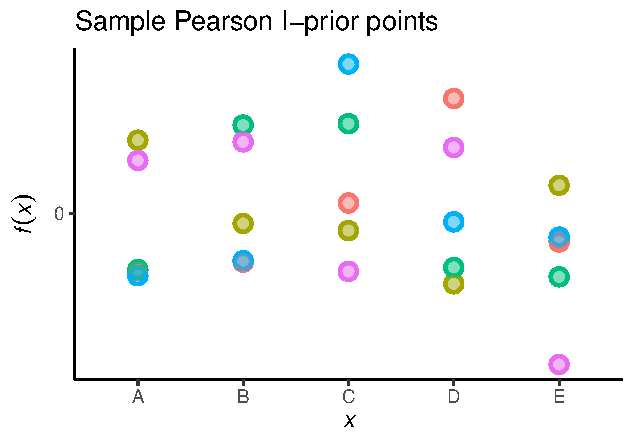
\includegraphics[width=0.53\textwidth]{figure/02-kernel_path_pearson}
  \caption[Sample I-prior ``paths'' from the Pearson RKHS]{Sample I-prior ``paths'' from the Pearson RKHS. These are represented as points over a finite set. Similarly coloured points are from the same ``path'', and since they are zero-mean functions, they sum to zero.}
\end{figure}



\section{Constructing RKKSs from existing RKHSs}\label{sec:constructrkks}

The previous section outlined all of the basic RKHSs of functions that will form the building blocks when constructing more complex function spaces.
As previously mentioned in the preliminaries, sums of kernels are kernels and products of kernels are also kernels. 
This provides us a platform for constructing new RKHS from existing ones.
To be more flexible in the specification of these new function spaces, we do not restrict ourselves to positive definite kernels only, thereby necessitating us to use the theory of RKKS.

\subsection{Sums, products and scaling of RKHS}

Sums of positive definite kernels are also positive definite kernels, and the product of positive definite kernel is a positive definite kernel.
They each, in turn, are associated with a RKHS that is defined by the sum of kernels and product of kernels, respectively.
The two lemmas below formalise these two facts. 

\begin{lemma}[Sum of kernels]\label{thm:sumkernels}
  If $h_1$ and $h_2$ are kernels on $\cX_1$ and $\cX_2$ respectively, then $h = h_1 + h_2$ is a kernel on $\cX_1 \times \cX_2$.
  Moreover, denote $\cF_1$ and $\cF_2$ the RKHS defined by $h_1$ and $h_2$ respectively.
  Then $\cF = \cF_1 \oplus \cF_2$ is an RKHS defined by $h = h_1 + h_2$, where
  \[
    \cF_1 \oplus \cF_2 = \{ f:\cX_1\times\cX_2 \to\bbR \,|\, f = f_1 + f_2, f_1\in\cF_1 \text{ and } f_2\in\cF_2 \}.
  \]
  For all $f\in\cF$,
  \[
    \norm{f}_\cF^2 = \min_{f_1+f_2=f} \left\{ \norm{f_1}_{\cF_1}^2 + \norm{f_2}_{\cF_2}^2 \right\}.
  \]
\end{lemma}

\begin{proof}
  That $h_1+h_2$ is a kernel should be obvious, as the sum of two positive definite functions is also positive definite.
  For a proof of the remaining statements, see \citet[Theorem 5]{berlinet2011reproducing}.
\end{proof}

\begin{lemma}[Products of kernels]\label{thm:prodkernels}
  Let $\cF_1$ and $\cF_2$ be two RKHS of functions over $\cX_1$ and $\cX_2$, with respective reproducing kernels $h_1$ and $h_2$.
  Then, $h = h_1 h_2$ is a kernel on $\cX_1 \times \cX_2$.
  Moreover, the tensor product space $\cF_1 \otimes \cF_2$ is an RKHS with reproducing kernel $h$.
\end{lemma}

\begin{proof}
  Fix $n\in\bbN$, and let $\bH_1$ and $\bH_2$ be the kernel matrices for $h_1$ and $h_2$ respectively.
  Since these kernel matrices are symmetric and positive-definite by virtue of $h_1$ and $h_2$ being symmetric and positive-definite functions, we can write $\bH_1 = \bA^\top\bA$ and $\bH_1 = \bB^\top\bB$ for some matrices $\bA$ and $\bB$: perform an (orthogonal) eigendecomposition of each of the kernel matrices, and take square roots of the eigenvalues.
  Let $\bH$ be the kernel matrix for $h = h_1h_2$.
  With $x_i = (x_{i1}, x_{i2})$, its $(i,j)$ entries are
  \begin{align*}
    h(x_i,x_j)
    &= h_1(x_{i1},x_{i2}) h_2(x_{j1},x_{j2}) \\
    &= (\bA^\top\bA)_{ij}\cdot (\bB^\top\bB)_{ij} \\
    &= \sum_{k=1}^n a_{ik}a_{jk} \sum_{l=1}^n b_{il}b_{jl},
  \end{align*}
  where we have denoted $b_{ij}$ and $c_{ij}$ to be the $(i,j)$th entries of $\bB$ and $\bC$ respectively 
  Then,
  \begin{align*}
    \sum_{i=1}^n\sum_{j=1}^n h(x_i,x_j)
    &= \sum_{k=1}^n \sum_{l=1}^n \sum_{i=1}^n \sum_{j=1}^n  \lambda_i \lambda_j a_{ik}a_{jk}b_{il}b_{jl} \\
    &= \sum_{k=1}^n \sum_{l=1}^n \left(\sum_{i=1}^n \lambda_i a_{ik} b_{il} \right) \left( \sum_{j=1}^n  \lambda_j a_{jk}b_{jl} \right) \\
    &= \sum_{k=1}^n \sum_{l=1}^n \left(\sum_{i=1}^n \lambda_i a_{ik} b_{il} \right)^2 \\
    &\geq 0
  \end{align*}
  Again, for the remainder of the statement in the lemma, we refer to \citet[Theorem 13]{berlinet2011reproducing}.
\end{proof}

A familiar fact from linear algebra is realised here from \cref{thm:sumkernels,thm:prodkernels}: 
%1) Multiplying a positive definite matrix by a positive constant results in a positive definite matrix; 
1) the addition of positive definite matrices is a positive definite matrix; and 
2) the \emph{Hadamard product}\footnotemark~of two positive definite matrices is a positive definite matrix.
\footnotetext{The Hadamard product is an element-wise multiplication of two matrices $\bA$ and $\bB$ of identical dimensions, denoted $\bA \circ \bB$. That is, $(\bA \circ \bB)_{ij} = \bA_{ij}\bB_{ij}$.}

The scale of an RKHS of functions $\cF$ over a set $\cX$ with kernel $h$ may be arbitrary.
To resolve this issue, a scale parameter $\lambda\in\bbR$ for the kernel $h$ may be introduced, which will typically need to be estimated from the data. 
If $h$ is a positive definite kernel on $\cX\times\cX$, and $\lambda \geq 0$ a scalar, then this yields a scaled RKHS $\cF_\lambda = \{\lambda f \,|\, f \in \cF \}$ with reproducing kernel $\lambda h$, where $\cF$ is the RKHS defined by $h$.

Restricting $\lambda$ to the positive reals is arbitrary and unnecessarily restrictive.
Especially when considering sums and products of scaled RKHSs, having negative scale parameters also give additional flexibility.
The resulting kernels from summation and/or multiplication with negative kernels may no longer be positive-definite, and in such cases, they give rise to RKKS instead.
%Obviously, a negative scale parameter implies that $\lambda h$ is negative-definite.
%Having negative scale parameters also give additional flexibility to polynomial and ANOVA RKKS, which we describe in the next subsections.
%An immediate consequence of having negative scale parameters is that sums and products of kernels may no longer be positive-definite.

\begin{remark}
  Recall that a RKKS $\cF$ of functions over $\cX$ can be uniquely decomposed as the difference between two RKHSs $\cF_+$ and $\cF_-$, and its associated Hilbert space $\cF_\cH$ is the RKHS $\cF_+ \oplus \cF_-$.
  If it is important to note that both $\cF$ and $\cF_\cH$  contain identical functions over $\cX$, but their topologies are different.
  That is to say, functions that are close with respect to the norm of $\cF$ may not be close to each other in the norm of $\cF_\cH$.
\end{remark}


%Without the positive restriction, the kernel may potentially be negative-definite.
%Therefore, the subsequent sections speak of RKKSs, instead of RKHSs, to account solely for the fact that $\lambda$ may be negative.
%All other properties of RKHSs should carry over to RKKSs, so sometimes we might overlook this distinction, and make references to RKHSs when instead RKKSs would be more suited to the context.
%\begin{remark}
%  As it turns out, for I-prior modelling, in cases where the RKHS is $\cF_\lambda$ with kernel $\lambda h$, then the sign of the single scale parameter $\lambda$ is unidentified.
%  Therefore, in such cases, we may restrict $\lambda\in\bbR^+$.
%  More on this in Chapter 4.
%\end{remark}
%Kreĭn spaces can be seen as a generalisation of Hilbert spaces, which caters for inner products not being positive definite.
%To motivate the need for Kreĭn spaces, we first look at several operations on reproducing kernels and the resulting vector space.
%\begin{lemma}[Scaling of kernels]\label{thm:scalingkernels}
%  If $h$ is a kernel on $\cX$, and $\lambda \geq 0$ a scalar, then $\lambda h$ is a kernel.
%  This yields a scaled RKHS $\cF_\lambda = \{\lambda f \,|\, f \in \cF \}$ with reproducing kernel $\lambda h$, where $\cF$ is the RKHS defined by $h$.
%\end{lemma}
%\begin{proof}
%  Multiplying a positive definite function by a positive constant results in a positive definite function still, and thus defines a unique RKHS.
%  The scaling of functions is seen through the fact that $\cF$ is the completion of the space spanned by the kernels, and hence $\cF_\lambda$ by the scaled kernels.
%\end{proof}
%The difference of kernels is not guaranteed to be a positive definite function.


\subsection{The polynomial RKKS}

A polynomial construction based on a particular RKHS building block is considered here.
For example, using the canonical RKHS in the polynomial construction would allow us to easily add higher order effects of the covariates $x \in \cX$.
In particular, we only require a single scale parameter in polynomial kernel construction.

\begin{definition}[The polynomial RKKS]
  Let $\cX$ be a Hilbert space.
  The kernel function $\hXXR$ obtained through the $d$-degree polynomial construction of linear kernels is
  \[
    h_\lambda(x,x') = \big(\lambda\cdot\ip{x,x'}_\cX + c\big)^d,
  \]
  where $\lambda \in \bbR$ is a scale parameter for the linear kernel, and $c \in \bbR$ is a real constant called the \emph{offset}.
  This kernel defined the \emph{polynomial RKKS} of degree $d$.
\end{definition}

Write
\begin{align*}
  h_\lambda(x,x')_\cF = \sum_{k=0}^d \frac{d!}{k!(d-k)!} c^{k-d} \lambda^k \ip{x,x'}_\cX^k.
%  &= \sum_{k=0}^d 
%  {\color{gray}\overbrace{\color{black}\frac{d!}{k!(d-k)!} c^{k-d} \lambda^k}^{\beta_k}}
%  \, \ip{x,x'}_\cX^k.
\end{align*}
Evidently, as the name suggests, this is a polynomial involving the canonical kernel.
In particular, each of the $k$-powered kernels (i.e., $\ip{x,x'}_\cX^k$) defines an RKHS of their own (since these are merely products of kernels), and therefore the sum of these $k$-powered kernels define the polynomial RKHS.

The offset parameter influences trade-off between the higher-order versus lower-order terms in the polynomial.
It is sometimes known as the bias term.

\begin{claim}
  The polynomial RKKS of functions over $\bbR$, denoted $\cF$, contains polynomial functions of the form $f(x)=\sum_{k=0}^d \beta_k x^k$.
\end{claim}

\begin{proof}
  By construction, $\cF = \cF_0 \oplus \bigoplus_{i=1}^d\bigotimes_{j=1}^i \cF_j$, where each $\cF_j, j \neq 0$ is the canonical RKHS, and $\cF_0$ is the RKHS of constant functions.
  Each $g \in \cF$ can therefore be written as $g = \beta_0 + \sum_{i=1}^d\prod_{j=1}^i f_j$, and $f_j(x)= b_j x$ from before, where $b_j$ is a constant.
  Therefore, $g(x) = \sum_{k=0}^d \beta_k x^k$.
\end{proof}

\begin{remark}
  We may opt to use other RKHSs as the building blocks of the polynomial RKHS.
  In particular, using the centred canonical kernel seems natural, so that each of the functions in the constituents of the direct sum of spaces is centred.
  However, the polynomial RKKS itself will not be centred.
\end{remark}


\subsection{The ANOVA RKKS}

We find it useful to begin this subsection by spending some time to elaborate on the classical \gls*{anova} decomposition, and the associated notions of main effects and interactions.
This will go a long way in understanding the thinking behind constructing an ANOVA-like RKKS of functions.

\subsubsection{The classical ANOVA decomposition}

The standard one-way ANOVA is essentially a linear regression model which allows comparison of means from two or more samples.
Given sets of observations $y_j = \{y_{1j},\dots,y_{n_jj}\}$, $j=1,\dots,m$, we consider the linear model $y_{ij} = \mu_j + \epsilon_{ij}$, where $\epsilon_{ij}$ are independent, univariate normal random variables with a common variance.
%One would like to test whether the hypothesis $\text{H}_0:\alpha_1=\cdots=\alpha_m$ stands.
%However, obtaining a suitable and significant test statistic to reject the null hypothesis merely tells us that the means are indeed not the same, but does not tell us \emph{where exactly} the difference lies.
%Enter the ANOVA decomposition.
This covariate-less model is used to make inferences about the  \emph{treatment means} $\mu_j$.
Often, the model is written in the \emph{overparameterised} form by substituting $\mu_j = \mu + \tau_j$.
This gives a different, arguably better, interpretability to the model: The $\tau_j$'s, referred to as the \emph{treatment effects}, now represent the amount of deviation from the grand, \emph{overall mean} $\mu$.
Estimating all $\tau_j$'s and $\mu$ separately is not possible because there is one degree of freedom that needs to be addressed in the model: There are $p+1$ mean parameters to estimate but only information from $p$ means.
%Knowledge of the overall mean $\mu$ would only allow us to freely ``choose'' only $m-1$ of the treatment effects $\mu_j$, since necessarily $\sum_{j=1}^m n_j\mu = \sum_{j=1}^m n_j\mu_j$.
A common fix to the identifiability issue is to set one of the $\mu_j$'s, say the first one $\mu_1$, to zero, or impose the restriction $\sum_{j=1}^m \mu_j = 0$.
The former treats one of the $m$ levels as the control, while the latter treats all treatment effects symmetrically.

%The imposition of these restriction corresponds to a particular hypothesis test regarding the group means.
%For instance, to test $\text{H}_0:\mu=\alpha_1=\cdots=\alpha_m$.

Now write the ANOVA model slightly differently, as $y_{i} = f(x_i) + \epsilon_{i}$, where $f$ is defined on the discrete domain $\cX = \{1,\dots,m\}$, and $i$ indexes all of the $n := \sum_{j=1}^m n_j$ observations.
Here, $f$ represents the group-level mean, returning $\mu_j$ for some $j\in\cX$.
In a similar manner, we can perform the ANOVA decomposition on $f$ as
\[
%  f = \greyoverbrace{Af}{f_0} +  \greyoverbrace{(I - A)f}{f_1},
  f = Af + (I-A)f = f_o + f_t,
\]
where $A$ is an averaging operator that ``averages out'' its argument $x$ and returns a constant, and $I$ is the identity operator.
$f_o = Af$ is a constant function representing the \textit{\underline{o}verall mean}, whereas $f_t = (I - A)f$ is a function representing the \textit{\underline{t}reatment effects} $\tau_j$.
Here are two choices of $A$:
\begin{itemize}
  \item $Af(x) = f(1) = \mu_1$. This implies $f(x) = f(1) + \big(f(x) - f(1)\big)$. The overall mean $\mu$ is the group mean $\mu_1$, which corresponds to setting the restriction $\mu_1=0$.
  \item $Af(x) = \sum_{x=1}^m f(x) / m =: \bar \alpha$. This implies $f(x) = \bar \alpha + \big( f(x) - \bar \alpha \big)$. The overall mean is $\mu = \sum_{j=1}^m \alpha_j/m$, which corresponds to the restriction $\sum_{j=1}^m \mu_j = 0$.
\end{itemize}
By definition, $AAf = A^2f = Af$, because averaging a constant returns that constant
[Side note: This idempotent property of the linear operator $A$ on $f$ speaks to the possibility of it being an \emph{orthogonal projection}, and indeed this is so---we shall return to this point later when we describe functional ANOVA decomposition].
We must have that $Af_t = A(I - A)f = Af - A^2f = 0$.
The choice of A is arbitrary, as is the choice of restriction, so long as it satisfies the condition that $Af_c = 0$.

The multiway ANOVA can be motivated in a similar fashion. 
Let $x = (x_1,\dots,x_p) \in \prod_{k=1}^p \cX_k$, and consider functions that map $\prod_{k=1}^p \cX_j$ to $\bbR$.
Let $A_j$ be an averaging operator on $\cX_k$ that averages the $k$th component of $x$ from the active argument list, i.e. $A_kf$ is constant on the $\cX_k$ axis but not necessarily an overall constant function.
An ANOVA decomposition of $f$ is
\[
  f = \left( \prod_{k=1}^p (A_k + I - A_k) \right)f = \sum_{\cK\in\cP_p} \left( \prod_{k\in\cK} (I - A_k) \prod_{k\notin\cK} A_k \right)f = \sum_{\cK\in\cP_p} f_\cK
\]
where we had denoted $\cP_p = \cP(\{1,\dots,p\})$ to be the power set of $\{1,\dots,p\}$ whose cardinality is $2^p$.
The summands $f_\cK$ will compose of the overall effect, main effects, two-way interaction terms, and so on.
Each of the terms will satisfy the condition $A_kf_\cK = 0, \forall k \in \cK \in \cP_p$.

\begin{example}[Two-way ANOVA decomposition]
  Let $p=2$, $\cX_1=\{1,\dots,m_1\}$, and $\cX_2=\{1,\dots,m_2\}$.
  The power set $\cP_2$ is $\big\{ \{\}, \{1\}, \{2\}, \{1,2\} \big\}$.
  The ANOVA decomposition of $f$ is
  \[
    f = f_0 + f_1 + f_2 + f_{12}.
  \]
  Here are two choices for the averaging operator $A_k$ analogous to the previous illustration in the one-way ANOVA.
  \begin{itemize}
    \item Let $A_1f(x) = f(1,x_2)$ and $A_2f(x) = f(x_1,1)$. Then,
    \begin{alignat*}{2}
      f_0 &= A_1A_2 f          &&= f(1,1) \\
      f_1 &= (I-A_1)A_2f       &&= f(x_1,1) - f(1,1) \\
      f_2 &= A_1(I-A2)f        &&= f(1,x_2) - f(1,1) \\
      f_{12} &= (I-A_1)(I-A2)f &&= f(x_1,x_2) - f(x_1,1) - f(1,x_2) + f(1,1).
    \end{alignat*}
    \item Let $A_kf(x) = \sum_{x_k=1}^{m_k} f(x_1,x_2) / m_k, k=1,2$. Then,
    \begin{alignat*}{2}
      f_0 &= A_1A_2 f          &&= f_{\bigcdot\bigcdot} \\
      f_1 &= (I-A_1)A_2f       &&= f_{x_1\bigcdot} - f_{\bigcdot\bigcdot} \\
      f_2 &= A_1(I-A_2)f        &&= f_{\bigcdot x_2} - f_{\bigcdot\bigcdot} \\
      f_{12} &= (I-A_1)(I-A_2)f &&= f - f_{x_1\bigcdot} - f_{\bigcdot x_2} + f_{\bigcdot\bigcdot},
    \end{alignat*}
    where $f_{\bigcdot\bigcdot} = \sum_{x_1,x_2} f(x_1,x_2) / m_1m_2$, $ f_{x_1\bigcdot} = \sum_{x_2} f(x_1,x_2)/m_2$, and \newline $f_{\bigcdot x_1} = \sum_{x_1} f(x_1,x_2)/m_1$.
  \end{itemize}
\end{example}

\subsubsection{Functional ANOVA decomposition}
\vspace{-5pt}
Let us now extend the ANOVA decomposition idea to a general function $f:\cX\to\bbR$ in some vector space $\cF$.
Specifically, we shall consider the (Hilbert) space of square integrable functions over $\cX$ with measure $\nu$, $\cF \equiv \text{L}^2(\cX,\nu)$.
We shall jump straight into the multiway ANOVA analogue for functional decomposition, and to that end, consider $x=(x_1,\dots,x_p) \in \prod_{k=1}^p \cX_k =: \cX$ a measurable space, where each of the spaces $\cX_k$ has measure $\nu_k$, and $\nu=\nu_1\times\cdots\times\nu_d$ is the product measure on $\cX$.
As $\cX$ need not necessarily be a collection of finite sets, we need to figure out a suitable linear operator that performs an ``averaging'' of some sort.

Consider the linear operator $A_k:\cF\to \cF_{-k}$, where $\cF_{-k}$ is a vector space of functions for which the $k$th component is constant over $\cX$, defined by
\begin{align}\label{eq:avgoper}
  A_k f = \int_{\cX_k} f(x_1,\dots,x_p) \dint \nu(x_k).
\end{align}
Thus, for the one-way ANOVA ($p=1$), we get
\begin{align}\label{eq:functionalanova1}
  f = 
  \greyoverbrace{\int_\cX f(x)\d\nu(x)}{f_0} 
  + 
  \greyoverbrace{\left( f - \int_\cX f(x)\d\nu(x) \right)}{f_1}
\end{align}
and for the two-way ANOVA ($p=2$), we have $f = f_0 + f_1 + f_2 + f_{12}$, with
\begin{align*}
  f_0 &= \int_{\cX_1}\int_{\cX_2} f(x_1,x_2) \dint\nu(x_1)\dint\nu(x_2) \\
  f_1 &= \int_{\cX_2} \left( f(x_1,x_2) - \int_{\cX_1} f(x_1,x_2) \dint\nu(x_1) \right) \dint\nu(x_2)\\  
  f_2 &= \int_{\cX_1} \left( f(x_1,x_2) - \int_{\cX_2} f(x_1,x_2) \dint\nu(x_2) \right) \dint\nu(x_1)\\  
  f_{12} &= f(x_1,x_2) - \int_{\cX_1} f(x_1,x_2) \d\nu(x_1) - \int_{\cX_2} f(x_1,x_2) \dint\nu(x_2) \\
  &\phantom{==} + \int_{\cX_1}\int_{\cX_2} f(x_1,x_2) \d\nu(x_1) \dint\nu(x_2).
\end{align*}

As a remark, the averaging operator $A_k$ defined in \cref{eq:avgoper} is indeed true to its name, in that it calculates the mean function of $f$ over the $k$th coordinate. 
For comparison, this is identical to the second type of restriction we considered in the classical ANOVA previously (i.e., setting $\sum_j \mu_j = 0$).
We must also have, as before, that $A_kf_\cK = 0, \forall k \in \cK \in \cP_p$.
For the one-way functional ANOVA decomposition in \cref{eq:functionalanova1}, it must be that $f_1$ is a zero-mean function.
As for the two-way ANOVA, it is the case that $\int_{\cX_k} f_1(x_1,x_2) \d\nu(x_k) = 0, k=1,2$, and $\int_{\cX_1}\int_{\cX_2} f_{12}(x_1,x_2) \d\nu(x_1)\d\nu(x_1) = 0$.

We notice that the decomposition in \cref{eq:functionalanova1} is orthogonal:

\begin{claim}
  For the ANOVA decomposition in \cref{eq:functionalanova1}, $f_0$ and $f_1$ are orthogonal for the usual $\text{L}^2$ inner product.
\end{claim}

\begin{proof}
  Note that $f_0$ is a constant function, and that $f_1 = f- f_0$.
  Thus,
  \begin{align*}
    \ip{f_0,f_1} 
    &= \int f_0f_1 \d\nu \\
    &= f_0 \int \left(f - f_0\right) \d\nu \\
    &= f_0 (f_0 - f_0) = 0.
  \end{align*}
\end{proof}

In fact, for $k=1$, any $f \in \cF$ can be decomposed as a sum of a constant plus a zero mean function, so we have the geometric decomposition of the vector space $\cF = \cF_0 \displaystyle\mathop{\oplus}^\bot \bar\cF_1$, where $\cF_0$ is a vector space of constant functions, and $\bar\cF_1$ a vector space of zero-mean functions over $\cX_1$.
For $k\geq 2$ we can argue something similar.
The space $\cF$ has the tensor product structure\footnotemark~$\cF = \cF_1 \otimes \cdots \otimes \cF_p$, and considered individually, each $\cF_k$ can be decomposed orthogonally $\cF_k = \cF_{0} \displaystyle\mathop{\oplus}^\bot \bar\cF_k$.
Note that $\cF_k$ consists of functions $f:\cX_k\to\bbR$.
Expanding out under the distributivity rule of tensor products and rearranging slightly, we obtain
\begin{align}
  \cF &= \big( \cF_0 \mathop{\oplus}^\bot \bar\cF_1 \big) \otimes \cdots \otimes 
  \big( \cF_0 \mathop{\oplus}^\bot \bar\cF_1 \big) \nonumber \\
  &= \cF_{0}^{\otimes p} 
  \ \mathop{\oplus}^\bot \
  \bigoplus_{j=1}^p \! \mathop{\vphantom\oplus}^\bot \Big( \cF_0^{\otimes (p-1)} \otimes \bar\cF_j \Big) 
  \ \mathop{\oplus}^\bot \
  \mathop{\bigoplus_{j,k=1}^p}_{j<k} \!\! \mathop{\vphantom\oplus}^\bot  \Big( \cF_0^{\otimes (p-2)} \otimes \bar\cF_j \otimes \bar\cF_k \Big)
  \label{eq:funcanovaspace} \\
  &\phantom{==} \mathop{\oplus}^\bot \ 
  \cdots 
  \ \mathop{\oplus}^\bot \ 
  \Big( \bar\cF_1 \otimes \cdots \otimes \bar\cF_p \Big). \nonumber
%  \\
%  &= \cF_0 
%  \mathop{\oplus}^\bot
%  \bigoplus_{j=1}^p \bar\cF_j
%  \mathop{\oplus}^\bot
%  \bigg( \mathop{\bigotimes_{j,k=1}^p}_{j<k} \bar\cF_j\bar\cF_k \bigg)
%  \mathop{\oplus}^\bot \ \cdots \ \mathop{\oplus}^\bot
%  \Big( \bar\cF_1 \otimes \cdots \otimes \bar\cF_p \Big).
\end{align}
To clarify,
\begin{itemize}
  \item $\cF_{0}^{\otimes p}$ is the space of constant functions $f:\cX_1\times\cdots\times\cX_p\to\bbR$.
  \item $\Big( \cF_0^{\otimes (p-1)} \otimes \bar\cF_j \Big)$ is the space of functions that are constant on all coordinates except the $j$th coordinate of $x$. Further, the functions are centred on the $j$th coordinate.
  \item $\Big( \cF_0^{\otimes (p-2)} \otimes \bar\cF_j \otimes \bar\cF_k \Big)$ is the space of functions that are constant on all coordinates except the $j$th and $k$th coordinate of $x$. Further, the functions are centred on these two coordinates.
  \item $\bar\cF_1 \otimes \cdots \otimes \bar\cF_p$ is the space of zero-mean functions $f:\cX_1\times\cdots\times\cX_p\to\bbR$.
  \item Similarly for the rest of the spaces in the summand, of which there are $2^p$ members all together. 
\end{itemize}

Therefore, given an arbitrary function $f\in\cF$, the projection of $f$ onto the above respective orthogonal spaces in \cref{eq:funcanovaspace} leads to the \emph{functional ANOVA representation}
\begin{align}\label{eq:functionalanova2}
  f(x) = \mu + \sum_{j=1}^p f_j(x_j) + \mathop{\sum_{j,k=1}^p}_{j<k} f_{jk}(x_j,x_k) + \cdots + f_{1\cdots p}(x).
\end{align}

\begin{definition}[Functional ANOVA representation]
  Let $\cP_d = \cP(\{1,\dots,d\})$, the power set of $\{1,\dots,d\}$.
  For any function $f \in \cF\equiv\text{L}^2(\cX_1\times\cdots\times\cX_d,\nu_1\otimes\cdots\otimes\nu_d)$, the formula for $f$ in \cref{eq:functionalanova2} is known as the \emph{functional ANOVA representation} of $f$ if $\forall k \in \cK \in \cP_p$,
  \begin{align}\label{eq:funcanovaorth}
    A_k f_\cK = \int_{\cX_\cK} f_\cK(x_\cK) \d\nu_k(x_k) = 0,
  \end{align}
  where $\cX_\cK = \prod_{k\in\cK} \cX_k$, and $x_\cK = \{x_k, k \in \cK \}$ is an element of this space.
  In other words, the integral of $f_\cK$ with respect to any of the variables indexed by the elements in $\cK$ (itself an element of the power set), is zero.
  The requirement \cref{eq:funcanovaorth} ensures orthogonality of the summands in \cref{eq:functionalanova2}.
\end{definition}

\footnotetext{There is an isomorphism $\text{L}^2(\cX_1\times\cdots\times\cX_d,\nu_1\otimes\cdots\otimes\nu_d) \cong \text{L}^2(\cX_1,\nu_1) \otimes \cdots \otimes \text{L}^2(\cX_d,\nu_d)$. See, for example, \citet{reed1972methods,kree1974produits}.}

For the constant term, main effects, and two-way interaction terms, the familiar classical expressions are obtained:
\begin{align*}
%  \mu &= \int%_\cX 
%  f(x) \d\nu(x) \\
%  f_j(x_j) &= \int%_{\prod_{i\neq j}\cX_i} 
%  f(x) \big( \textstyle\prod_{i\neq j} \d\nu_i(x_i) \big) - \mu \\
%  f_{jk}(x_j,x_k) &= \int%_{\prod_{i\neq j,k}\cX_i} 
%  f(x) \big( \textstyle\prod_{i\neq j,k} \d\nu_i(x_i) \big) - f_j(x_j) - f_k(x_k) - \mu  
  f_0 &= \int f \d\nu \\
  f_j &= \int f \, \textstyle\prod_{i\neq j} \d\nu_i  - f_0 \\
  f_{jk} &= \int f \, \textstyle\prod_{i\neq j,k} \d\nu_i  - f_j - f_k - f_0  .
\end{align*}

%Any function square integrable function $f$ can be decomposed as a sum of a constant plus a zero mean function.

%The two elements are orthogonal for the usual $\text{L}^2$ inner product $\ip{f,g} = \int_\cX f(x)g(x)\d\nu(x)$.
%Therefore, we have a geometric decomposition 
%\[
%  \cF = \cF_0 \oplus \bar\cF
%\]
%where $\cF_0$ is the subspace of constant functions, and $\bar\cF$ is the subspace of zero mean functions: $\bar\cF = \{f \in \cF | \int_\cX f\d\nu = 0 \}$.

\begin{remark}
  Not all of the higher order terms need to be included. There may even be a model motivated reason for dropping certain main effects or interaction effects.  
\end{remark}


\subsubsection{The ANOVA kernel}

At last, we come to the section of deriving the ANOVA RKKS, and, rest assured, the preceding long build-up will prove to be not in vain.
The main idea is to construct an RKKS such that the functions that lie in them will have the ANOVA representation in \cref{eq:functionalanova2}.
The bulk of the work has been done, and in fact we know exactly how this ANOVA RKKS should be structured---it is the space as specified in \cref{eq:funcanovaspace}. 
The ANOVA RKKS will be constructed by a similar manipulation of the individual kernels representing the RKHS building blocks.

\begin{definition}[The ANOVA RKKS]\label{def:anovarkks}
  For $k=1,\dots,p$, let $\cF_k$ be a centred RKHS of functions over the set $\cX_k$ with kernel $h_k:\cX_k\times\cX_k\to\bbR$. 
  Let $\lambda_k, k=1,\dots,p$ be real-valued scale parameters.
  The ANOVA RKKS of functions $f:\cX_1\times\cdots\times\cX_p\to\bbR$ is specified by the ANOVA kernel, defined by
  \begin{align}\label{eq:anovarkks}
    h_\lambda(x,x') = \prod_{k=1}^p \big( 1 + \lambda_k h_k(x_k,x_k') \big).
  \end{align}
\end{definition}

The construction an ANOVA RKKS is very very simple in through multiplication of univariate kernels.
Expanding out equations \cref{eq:anovarkks}, we see that it is in fact a sum of products of kernels with increasing orders of interaction:
\begin{align*}
  h_\lambda(x,x') 
%  &= \prod_{k=1}^p \big( 1 + \lambda_k h_k(x_k,x_k') \big) \\
  &= 1 + \sum_{j=1}^p \lambda_j h_j(x_j,x_j') + \mathop{\sum_{j,k=1}^p}_{j<k} \lambda_j\lambda_k h_j(x_j,x_j')h_k(x_k,x_k') \\
  &\phantom{==} + \cdots + \prod_{j=1}^p \lambda_j h_j(x_j,x_j').
\end{align*}
It is now clear from the expansion that the ANOVA RKKS yields functions that resemble those with the ANOVA representation in \cref{eq:functionalanova2}:
The mean value of the function stems from the `1', i.e. it lies in an RKHS of constant functions; the main effects are represented by the sum of the individual kernels; the two-way interaction terms are represented by the second-order kernel interactions; and so on.

%One thing to note is that restricting the $\lambda$ parameters to the positive orthant might give unsatisfactory results---what if the effect of two functions are in truth opposing one another?
%These are handled through opposing signs of their respective scale parameters, thus  the need for working in RKKSs.

\begin{example}
  Consider two RKKSs $\cF_k$ with kernel $\lambda_k h_k$, $k=1,2$.
  The ANOVA kernel defining the ANOVA RKKS $\cF$ is
  \[
    h_\lambda\big((x_1,x_2),(x_1',x_2') \big) = 1 + \lambda_1 h_1(x_1,x_1') + \lambda_2 h_2(x_2,x_2') + \lambda_1\lambda_2 h_1(x_1,x_1')h_2(x_2,x_2').
  \]  
  Suppose that $\cF_1$ and $\cF_2$ are the centred canonical RKKS of functions over $\bbR$.
  Then, functions in $\cF = \cF_0 \oplus \cF_1 \oplus \cF_2 \oplus (\cF_1 \otimes \cF_2)$ are of the form
  \[
    f(x_1,x_2) = \beta_0 + \beta_1x_1 + \beta_2x_2 + \beta_3x_1x_2.
  \]
\end{example}

As remarked in the previous subsection, not all of the components of the ANOVA RKKS need to be included in the construction.
The selective exclusion of certain interactions characterises many interesting statistical models.
Excluding certain terms of the ANOVA RKKS is equivalent to setting the scale parameter for those relevant components to be zero, i.e., they play no role in the decomposition of the function.
With this in mind, the ANOVA RKKS then gives us an objective way of model-building, from linear regression, to multilevel models, longitudinal models, and so on.
%One thing's for sure---everything is ANOVA.

%\begin{remark}
%  Unfortunately, even if centred RKHSs are used as the building blocks of the ANOVA RKKS, the properties of the function represented by \cref{eq:functionalanova2} may not be preserved.
%  In particular, any of the individual functions $f_\cK$, for $\cK$ in the power set, are not necessarily zero mean functions.
%  Furthermore, any two terms in the summand are generally not orthogonal.
%  \hltodo[What are advantages of using ANOVA? I feel this has not been addressed properly.]{Consequently, interpretation based on an ANOVA motivation may not be valid, but in spirit, they provide a conceptually strong basis for building new RKKSs from existing ones.}
%\end{remark}



\section{Summary}\label{sec:summarychapter2}

The review of functional analysis allows us to describe the theory of RKHSs and RKKSs, which are of interest to us because the topology endowed on such spaces gives appreciable assurances---in particular, all evaluation functionals are continuous in these spaces.
Moreover, RKHSs and RKKSs can be specified completely through kernel functions, with new and complex function spaces built simply by manipulation of these kernel functions.
Of particular importance is the ANOVA functional decomposition, for which we realise provides an objective way of constructing various function spaces for regression and modelling. 
Such models will be described later on in detail in \cref{chapter4}.

An annotated collection of bibliographical references used for this chapter is as follows.
\begin{itemize}
  \item \textbf{Functional analysis}. 
  On the introductory material relating to functional analysis in \cref{sec:funcanalysis}, the lecture notes by \citet{sejdinovic2012} is recommended, and forms the basis for most of our material. 
  Additionally, \citet{rudin1987real,yamamoto2012vector,kokoszka2017introduction} provides a complementary reading.
  \item \textbf{RKHS theory}. 
  There are certainly no shortages of introductory texts relating to the theory of RKHS: \citet{steinwart2008support}, \citet{berlinet2011reproducing}, and \citet{gu2013smoothing} to name a few. 
  The concise sketch proof for the Moore-Aronszajn theorem was mostly inspired by \citet[Theorem 4]{hein2004kernels}.
  \item \textbf{RKKS theory}. 
  The innovation of indefinite inner product spaces perhaps started in mathematical physics literature, for which the theory of special relativity depends. 
  Four-dimensional space-time is an often cited example. 
  In any case, we referred to mainly \citet{ong2004learning}, which gives an overview in the context of learning using indefinite kernels. 
  \citet{alpay1991some} and \citet{zafeiriou2012subspace} were also useful for understanding the fundamental concepts of RKKS.
  \item \textbf{RKHS building blocks}. 
  The main building block RKHS, i.e. the canonical RKHS, the fBm RKHS and the Pearson RKHS are described in the manuscript of \citet{bergsma2017}.
  \item \textbf{ANOVA and functional ANOVA}. 
  Classical ANOVA is pretty much existent in every fundamental statistical textbook. These texts have extremely well written introductions to this very important concept: \citet[Ch. 11]{casella2002statistical}, \citet[Ch. 3]{dean1999design}. 
  On the relation between classical ANOVA and functional ANOVA decomposition, \citet{gu2013smoothing} offers novel insights. There is diverse literature concerning functional ANOVA, namely from the fields of statistical learning (e.g. \cite{wahba1990spline}), applied mathematics (e.g. \cite{kuo2010decompositions}), and sensitivity analysis (e.g. \cite{sobol2001global,durrande2013anova}). 
%  What is interesting is that several authors who simply set out to obtain a suitable functional decomposition, all ended up somewhat independently recovering the ANOVA decomposition as being ``optimal'' in some sense.
%  This speaks largely to this classical idea that is ANOVA.
\end{itemize}


\hClosingStuffStandalone
\end{document}